\documentclass[a4paper, 14pt]{extarticle}

\usepackage[english]{babel}
\usepackage[utf8x]{inputenc}
\usepackage[T1]{fontenc}
\newtheorem{theorem}{Theorem}
\usepackage[a4paper,top=2.9cm,bottom=2.9cm,left=3cm,right=3cm,marginparwidth=2cm]{geometry}
\usepackage{amsmath}
\usepackage{graphicx}
\usepackage{lscape}
\usepackage[colorinlistoftodos]{todonotes}
\usepackage[colorlinks=true, allcolors=blue]{hyperref}
\usepackage{float}
\usepackage{url}
\usepackage{palatino}
\usepackage[ruled,vlined]{algorithm2e}
\restylefloat{table}


\title{tPerformance Study of Extreme Learning Machines}
\author{Wanli Huang}
\begin{document}
\maketitle
\newpage
\tableofcontents

\newpage
\begin{abstract}
\par The Extreme Learning Machine (ELM) is a new Machine Learning methodology that has appeared relatively recently, and is very promising according to its authors, as it is quite simple and elegant. The ELM is essentially a learning model that consists of only a single hidden layer feedforward neural network (SLFN). A conventional SLFN network is a gradient-based algorithm that uses the backpropagation (BP) learning strategy. ELMs use minimum norm least-squares solutions by contrast. Some researchers on ELMs claim that ELMs are faster, provide better performance and are more reliable than SLFNs using the traditional BP learning algorithm. The goal of this thesis is to present a study on ELM algorithms, to verify their performance comparing them with other state-of-the-art machine learning methods.
%\par Extreme Learning Machines (ELMs) emerge relatively recently and seem promising. They present as elegant and simple algorithms. ELMs are a kind of single hidden layer feedforward neural network (SLFN). A conventional SLFN is gradient-based and uses the backpropagation (BP) learning algorithms. ELMs use minimum norm least-squares solutions by contrast. Many researchers on ELMs claim that ELMs have faster speed, better performance and are more reliable than SLFN that uses the traditional BP learning algorithm. The goal of this thesis is to study ELM algorithms, verify the claims and evaluate them by comparison with other mature machine learning methods such as Hoeffding Tree. 
\par We built two major implementations to evaluate the ELM methodology. The first, named \emph{basic ELM}, is implemented within the WEKA framework to perform experiments in the batch data mining setting. The second, named \emph{Online Sequential ELM}, is implemented within the MOA framework to do experiments in the streaming data mining setting. 
\par The experiments show that the basic ELM WEKA implementation does not achieve the same performance as claimed by ELM authors. The Online Sequential ELM MOA version does not have better performance than state-of-the-art methods such as the Hoeffding Tree or the Hoeffding Adaptive Tree. One of the main discoveries of this thesis is that the number of neural units in the hidden layer determines the accuracy and learning speed and that ELMs may be suitable only for medium to small size datasets. 

%\par To verify and evaluate the ELM, two major implementations were completed. The first is called basic ELM, which is implemented within the WEKA framework to do experiments in the static data setting. The second is called Online Sequential ELM, which is implemented within the MOA framework to do experiments in the streaming data setting. 
%\par The experiments show that basic EML WEKA version doesn't get the same good performance as the claims. Online Sequential ELM MOA version doesn't have better performance than HoeffdingTree or HoeffdingAdaptiveTree. The number of neutral unit of the hidden layer determines the accuracy and the learning speed. ELMs are suitable for medium to small size dataset. 
\end{abstract}
\newpage
\section{Introduction}
\par Machine learning techniques have successfully demonstrated their promising potential in many applied applications. There are many different categories of machine learning techniques, among which, feedforward neural networks (FNNs) have been widely and extensively applied in different domains. One of the important capabilities of FNNs is their universal approximation capabilities. G. Cybenko and K. Hornik both investigated the simplest FNN, which only has one single hidden neuron units layer, the so-called Single Hidden Layer Feedforward Neural Network (SLFN). G. Cybenko showed the approximation properties in his paper that: "arbitrary decision regions can be arbitrarily well approximated by continuous feedforward neural networks with only a single internal hidden layer and any continuous sigmoidal nonlinearity" \cite{Cybenko1989ApproximationBS}. K. Hornik also proved the universal approximation capabilities of standard FNNs with one single hidden layer and different types of nonlinearity (nonconstant) activation functions when the hidden units are sufficient\cite{HORNIK1991251}. 

G.B. Huang and HA Babri also proved that SLFNs with sufficient hidden neurons and with almost any bounded nonlinear activation function could learn distinct observations with zero error\cite{655045} \cite{G.B.Huang-ICNN}. The universal approximation capability allows FNNs to be trained on a finite sample set, and then the continuous mapping can be learned from it\cite{HORNIK1991251}. Researchers have proposed many learning algorithms, among which the most popular and successful is the gradient-based backpropagation algorithm. DE Rumelhart, G.E Hilton and R.J Williams describe a learning procedure called backpropagation (BP) for feedforward neural networks. The BP algorithm repeatedly adjusts input weights of the FNNs to find the best input weights that can minimize the difference between the actual output results and the expected output results\cite{rumelhart1988learning}. There are other learning methods such as the Orthogonal least squares learning algorithm\cite{Chen1991OrthogonalLS} and the Marquardt algorithm\cite{hagan1994training}. This paper focuses on SLFNs to keep it as simple as possible.
\par Regarding the use of the BP learning algorithm to train SLFNs, G.B. Huang et al. argued that there are some issues\cite{G.B.Huang-ICNN}\cite{6035797}\cite{huang2006extreme}: \begin{itemize}
    \item Learning rate plays an important role in learning. If the learning rate is too low, it converges very slowly. If the learning rate is too high, the learning process is unstable and not easy to converge. As a result, it is important to find proper learning steps. 
    \item It is easy for the BP algorithm to converge to local minima. If the local minimum is far away from the global minimum, the mapping results of the SLFN are not desirable.
    \item It is an iterative algorithm which is time-consuming.
    \item To prevent it from being over-trained, validation and early stopping techniques are applied, which make the SLFNs learning process more complex. 
\end{itemize} 
For solving these issues, a simple, promising learning algorithm called Extreme Learning Machine(ELM) was proposed by G.B. Huang in 2005. The ELM is based on artificial feedforward neural networks, especially Single Hidden Layer Feedforward Neural Networks (SLFNs). The structure of a standard ELM is a single hidden layer feedforward neural network with input weights from the input layer to the hidden layer and trainable output weights from the hidden layer to the output layer. There is also a bias vector input to the hidden layer. There are several features of the ELM\cite{huang2015extreme}: 
\begin{itemize}
    \item The input weights are initialized randomly, as well as the bias parameters. 
    \item There is no need to tune input weights and bias parameters. 
    \item There is no iterative process when training the output weights. The output weights can be calculated in a single batch step. 
    \item The training method uses the minimum norm least-squares solution.
\end{itemize}
ELMs have been applied in two major data set scenarios: the static data setting and the stream data setting. As a result, various ELMs have been developed. Like other machine learning methods, ELMs perform classification and regression tasks. Figure \ref{fig:machine learning} shows the ELM family within the scope of machine learning methods. 
\begin{figure}[H]
\centering
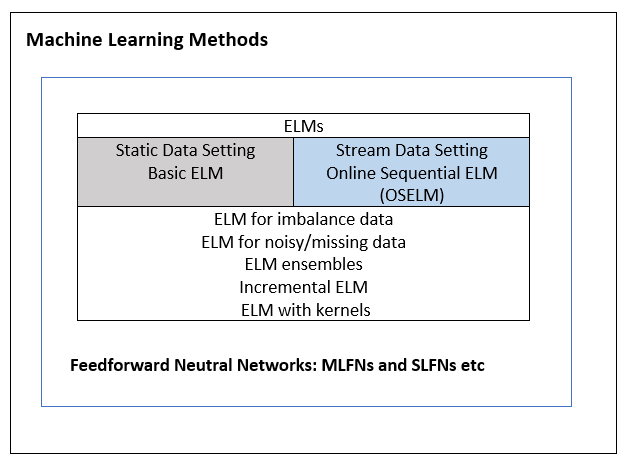
\includegraphics[width=\textwidth]{1.png}
\caption{\label{fig:machine learning}ELM Family}
\end{figure}
ELM researchers claim that ELMs train faster as well as produce better accuracy results compared to the BP learning algorithm and other machine learning methods. \newline
\par  \textit{The goal of this thesis is to examine and evaluate ELM learning algorithm performance on classification tasks as well as to find out how ELMs can be applied in a data stream setting. Three aspects are covered: speed, accuracy and reliability, accuracy is the main focus.} \newline
\par This thesis looks at two variants of the ELM. The first is the basic ELM\cite{G.B.Huang-ICNN}, which is implemented within the WEKA framework\cite{frank2009weka}, to investigate the performance and other aspects in a static data setting. The second is the Online Sequential ELM\cite{liang2006fast}, which is implemented within the MOA framework\cite{bifet2010moa}, to investigate how the ELM is applied in a data stream setting. Additionally, both implementations are used to conduct experiments on different datasets. 
\par This thesis is organized as follows. Section 2 reviews some related work. SLFN, the BP algorithm, basic ELM, Online Sequential ELM, other types of ELM and related theorems are discussed in this section. Section 3 describes the implementations within the WEKA framework and the MOA framework. Section 4 presents the experiments and the results and provides the performance, speed and reliability evaluations with a focus on performance. 
\newpage
\section{ Review of related work}
The Extreme Learning Machine is a kind of learning algorithm for artificial feedforward neural networks. A review of related work is presented in this section. Firstly, some related theorems supporting ELMs are introduced. Secondly, Single Hidden Layer Feedforward Neural Networks (SLFNs) and the conventional backpropagation learning algorithm are discussed. Thirdly, the basic Extreme Learning Machine algorithms are focused on. Fourthly, the Online Sequential ELM in streaming data setting is investigated as well. Lastly, some variants of ELM and their application are also reviewed. 
\subsection{Related Theorems}
ELMs are based on several theorems. If the activation function \(g\) is infinitely differentiable, the number of hidden neuron nodes \(L\) should be smaller than the number of instances. This can be proved in the following two theorems.  
\par 
\begin{theorem}
Given a standard SLFN with \(L\) hidden nodes, and an activation function \(g\) which is infinitely differentiable in any interval, for \(N\) distinct samples/instances \((\mathbf{x_i, t_i})\) where \(\mathbf{x}_i \in \mathbf{R}^n\) and \(\mathbf{t}_i \in \mathbf{R}^m\). For any \(\mathbf{w}_i\) and \(b_i\) randomly chosen from any intervals of \(\mathbf{R}^n\) and \(\mathbf{R}\). Respectively, according to any continuous probability distribution, then with probability one, the hidden layer output matrix \(\mathbf{H}\) of the SLFN is invertible and \(\Vert\mathbf{H}\beta - \mathbf{T}\Vert = 0\)\cite{huang2006extreme}. 
\end{theorem}
(For \(\mathbf{H}\) and \(\mathbf{T}\) definitions, refer to Equation 9, section 2.3)
\begin{theorem}
Given any small positive value \(\epsilon>0\) and activation function \(g\) which is infinitely differentiable in any interval, there exists \(L \leq N \) such that for \(N\) arbitrary distinct samples \((\mathbf{x_i, t_i})\) where \(\mathbf{x}_i \in \mathbf{R}^n\) and \(\mathbf{t}_i \in \mathbf{R}^m\). For any \(\mathbf{w}_i\) and \(b_i\) randomly chosen from any intervals of \(\mathbf{R}^n\) and \(\mathbf{R}\). Respectively, according to any continuous probability, then with probability one, \(\parallel \mathbf{H}_{N \times L}\beta_{L \times m} - \mathbf{T}_{n \times m}\parallel < \epsilon \)\cite{huang2006extreme}
\end{theorem}
(For \(\mathbf{H}\) and \(\mathbf{T}\) definitions, refer to Equation 9, section 2.3)\newline
\par These two theorems prove that for any activation function with a continuous probability distribution, we can make the column vector of \(\mathbf{H}\) full rank so long as \(\mathbf{H}\) is invertible. Providing the number of instances is larger than the number of hidden neuron nodes, the ELM can be trained to find the global minimum error. To find the global minimum error, the Moore-Penrose generalized inverse and the minimum norm least-squares solution of a general linear system provide the theoretical support. 
\begin{theorem}
Moore-Penrose generalized inverse\cite{banerjee1973generalized}\cite{serre2010matrices}
\par For a linear equation \(\mathbf{Ax} = \mathbf{y}\), where \(\mathbf{A}\) is of order  \(m\times n \), which may be singular and may not be square, there is a matrix \(\mathbf{G}\) of order \(n\times m \) called the Moore-Penrose generalized inverse of the matrix \(\mathbf{A}\), if the following equations are satisfied:\newline \par  \(\mathbf{AGA} = \mathbf{A}\), \(\mathbf{GAG} = \mathbf{G}\), \(\mathbf{(AG)}^T = \mathbf{AG}\), \(\mathbf{(GA)}^T = \mathbf{GA}\)
\newline\newline The Moore-Penrose generalized inverse of matrix \(\mathbf{A}\) can be denoted by \(\mathbf{A}^\dagger\). 
\end{theorem}
\begin{theorem}
Minimum norm least-squares solution of a general linear system\cite{G.B.Huang-ICNN}
\par For a general linear system \(\mathbf{Ax} = \mathbf{y}\), if there is \(\hat{\mathbf{x}}\) satisfying:
\newline \par \(\Vert\mathbf{A\hat{x}}-\mathbf{y}\Vert =  \min_{x}\Vert\mathbf{Ax}-\mathbf{y}\Vert\)
\newline\newline
then \(\hat{\mathbf{x}}\) is a least-squares solution. Where \(\Vert\cdot\Vert\) is a norm in Euclidean space. If a solution \(\mathbf{x}_0\) is the smallest norm among all the least-squares solutions, then \(\mathbf{x}_0\) is the minimum norm least-squares solution of the linear system \(\mathbf{Ax} = \mathbf{y}\). 
\end{theorem}
\begin{theorem}
According to \cite{G.B.Huang-ICNN}\cite{serre2010matrices}, if there is a matrix \(\mathbf{G}\) to make \(\mathbf{Gy}\) be a minimum norm least-squares solution of a linear system \(\mathbf{Ax} = \mathbf{y}\), then \(\mathbf{G}\) is necessary and sufficient to be the Moore-Penrose generalized inverse of \(\mathbf{A}\), denoted by \(\mathbf{A}^\dagger\).   
\end{theorem}
\subsection{SLFN and BP algorithm}
\subsubsection{SLFN structure}
\par A feedforward neural network (FNN) is a kind of artificial neural network, where the input information flows only in one direction from the input layer, through other layers and finally to the output layer. A layer is a set of neural nodes. There are no cycles or feedback loops in the network\cite{Goodfellow-et-al-2016}\cite{witten2016data}. Single Hidden Layer Feedforward Neural Network(SLFN) is a focus as it is the simplest and most complete FNN. 
\par The structure of SLFN is made of three layers: an input layer, a hidden layer and an output layer. Figure \ref{fig:SLFN} shows a typical SLFN structure \cite{witten2016data}. 
\begin{figure}[H]
\centering
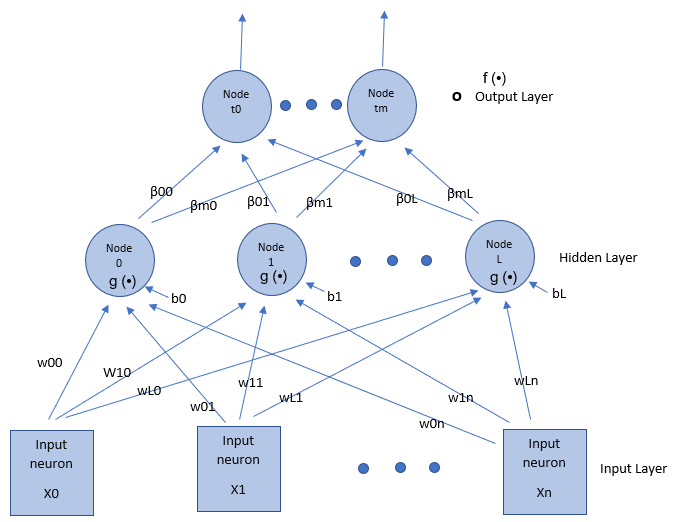
\includegraphics[width=\textwidth]{SLFN.png}
\caption{\label{fig:SLFN}Single Hidden Layer Feedforward Neural Network Structure}
\end{figure}
\begin{itemize}
    \item 
 \( (x_1, x_2, ..., x_n)\) represents each feature of an instance. There are \(n\) features. Each feature is an input to a neural unit. The number of neural units in the input layer is the number of features of an instance. 
 \item The hidden layer has \(L\) neuron nodes. Each input neuron node is connected to each hidden neuron node. \( w_{ij} \) is the input weight for each connection between the input neuron nodes and the hidden neuron node. \( i= 1, ..., L.   j = 1, ..., n.  \) 
 \item \(\beta_{ki}\) is the output weight from each hidden neuron node to each output neuron node. \( k=1, ..., m.   i= 1, ..., L. \)
 \item \( t_0, t_1, ..., t_m\) are the labels of the class of the instance. The number of label is the number of neuron node of output layer. 
 \item \( b_0, b_1, ..., b_L\) are the bias input to each hidden neuron node. 
 \item \( g(\cdot) \) is an activation function. 
 \item \(\mathbf{o}\) is the predicted label vector of the output. 
\end{itemize}
\par 
\subsubsection{Back-propagation learning algorithm}
\par The BP learning algorithm is quite popularly applied on the SLFN. The target of BP is to minimize the cost function between the predicted results and the actual results. 
\par Each instance has \(n\) features and a class \(t\), each class \(t\) has \(m\) labels. For \(N\) distinct instances \((\mathbf{x_i}, \mathbf{t_i})\), where \(\mathbf{x_i} = [x_{i1}, x_{i2}, ..., x_{in}]^T , i = 1, 2, ..., N\) and \(\mathbf{t_i} = [t_{i1}, t_{i2}, ..., t_{im}]^T , i = 1, 2, ..., N\) \cite{G.B.Huang-ICNN}
\par For a standard SLFN in Figure 2, there are \(L\) hidden neuron nodes, and the activation function is \(g(x)\), the machine learning model is\cite{G.B.Huang-ICNN} 
\begin{equation}
  \sum_{k=1}^L{\beta_k}g(\mathbf{w}_k \cdot \mathbf{x}_i + b_k) = \mathbf{o}_i,  i = 1, 2, ..., N
\end{equation}
where \( \mathbf{w}_k = [w_{k1}, w_{k2}, ..., w_{kn}]^T \) are the input weights and \( \mathbf{\beta}_k = [\beta_{k1}, \beta_{k2}, ..., \beta_{km}]^T \) are the output weights and \(b_k\) is the bias value of the \(k\)th hidden neuron node. \(\mathbf{o}_i\) is the \(i\)th instance's predicted class value. 
\par For a training dataset, the class values of each training instance are known as \(\mathbf{t}\), where \(\mathbf{t_i} = [t_{i1}, t_{i2}, ..., t_{im}]^T , i = 1, 2, ..., N\). The calculation of actual results is \cite{G.B.Huang-ICNN}
\begin{equation}
  \sum_{k=1}^L{\beta_k}g(\mathbf{w}_k \cdot \mathbf{x}_i + b_k) = t_i,  i = 1, 2, ..., N
\end{equation}
\par Zero error between the results of Equation(1) and Equation(2) is expected, which means for \(N\) instances, the SLFN needs to be trained to achieve
\begin{equation}
    \sum_{i=1}^N\parallel \mathbf{o}_i - \mathbf{t}_i \parallel = 0
\end{equation}
\par Equally, the SLFN can be trained to find the optimized output weights by minimizing the cost function
\begin{equation}
    E = \sum_{i=1}^N\bigg(\sum_{k=1}^L\beta_kg(\mathbf{w}_k \cdot \mathbf{x}_i+ b_k)-\mathbf{t}_i\bigg)^2
\end{equation}
Equation (4) can be also written as \( E = F(\mathbf{W})\), where vector \( \mathbf{W}\) is the set of weights\((\mathbf{w}_k, \beta_k)\) and bias \(b_k\) parameters\cite{G.B.Huang-ICNN}. The goal of training the SLFN is to find optimized \(\mathbf{W}\), which can be adjusted iteratively by using a gradient-based algorithm as follows\cite{G.B.Huang-ICNN}: 
\begin{equation}
    \mathbf{W}_t = \mathbf{W}_{t-1} - \eta\frac{\partial F(\mathbf{W})}{\partial \mathbf{W}}
\end{equation}
Where $\eta$ is a learning rate. After each layer's output value is calculated from the input layer to the output layer, Equation (5) allows gradients to be worked out easily by backpropagation from the output to the input to adjust the \(\mathbf{w}\) and \(\beta\) parameters until the cost function is minimized. 
\par As mentioned in the last section, there are some issues with the BP learning algorithm. The Extreme Learning Machine was proposed to solve these problems.
\subsection{Extreme Learning Machine (ELM)}
\subsubsection{Principle of ELM} 
\par In this section, the principle of ELM is investigated. An ELM is an SLFN. To simplify the discussion, we can rewrite Equation (2) as the following equation\cite{huang2006extreme}:
\begin{equation}
    \mathbf{H}\beta = \mathbf{T}
\end{equation}
where 
\begin{equation}
\begin{split}
    &\mathbf{H}(\mathbf{w_1, ..., w_L},  b_1, ..., b_L, \mathbf{x_1, ..., x_N})\\&=
    \begin{bmatrix}
    g(\mathbf{w_1 \cdot x_1} + b_1) & \cdots & g(\mathbf{w_L \cdot x_1} + b_L)\\
    \cdot & \cdots & \cdot\\
    \cdot & \cdots & \cdot\\
    \cdot & \cdots & \cdot\\
    g(\mathbf{w_1 \cdot x_N} + b_1) & \cdots & g(\mathbf{w_L \cdot x_N} + b_L)
    \end{bmatrix}_{N\times L}
\end{split}
\end{equation}
\newline
\begin{equation}
    \beta =
    \begin{bmatrix}
    &\beta_1^T&\\
    &\cdot&\\
    &\cdot&\\
    &\cdot&\\
    &\beta_L^T&
    \end{bmatrix}_{L \times m}
\end{equation}
\newline
\begin{equation}
    \mathbf{T} =
    \begin{bmatrix}
    &\mathbf{t}_1^T&\\
    &\cdot&\\
    &\cdot&\\
    &\cdot&\\
    &\mathbf{t}_N^T&
    \end{bmatrix}_{N \times m}
    =
    \begin{bmatrix}
    t_{11} & \cdots & t_{1m}\\
    \cdot & \cdots & \cdot\\
    \cdot & \cdots & \cdot\\
    \cdot & \cdots & \cdot\\
    t_{N1} & \cdots & t_{Nm}
    \end{bmatrix}_{N \times m}
\end{equation}
and \(N\) is the number of instances. \(L\) is the number of hidden neuron nodes. \(m\) is the number of labels of the class, as well as the number of output neuron nodes.
\par \textbf{H} is called the hidden layer output matrix of the SLFN. The \(i\)th column of \textbf{H} is the \(i\)th hidden neuron node output with respect to each instance of \(\mathbf{x}_1, \mathbf{x}_2, ..., \mathbf{x}_N\)\cite{huang2006extreme}. As a result, \(\mathbf{H}\) can be also written much more compactly as follows. 
\begin{equation}
    \mathbf{H}
    =
    \begin{bmatrix}
    &\mathbf{h(x_1)}&\\
    &\cdot&\\
    &\cdot&\\
    &\cdot&\\
    &\mathbf{h(x_N)}&\\
    \end{bmatrix}_{N \times L}
    = 
    \begin{bmatrix}
    h_1(\mathbf{x}_1) & \cdots & h_L(\mathbf{x}_1)\\
    \cdot & \cdots & \cdot\\
    \cdot & \cdots & \cdot\\
    \cdot & \cdots & \cdot\\
    h_1(\mathbf{x}_N) & \cdots & h_L(\mathbf{x}_N)\\
    \end{bmatrix}_{N\times L}
\end{equation}
From Equation (7) and Equation (10), each hidden neuron nodes output regarding to each instance is written as:  
\begin{equation}
    h_i(\mathbf{x}) = G(\mathbf{w_i}, b_i, \mathbf{x_i})
\end{equation}
\(G(\mathbf{w_i}, b_i, \mathbf{x_i})\) can use the following activation functions to map the input domain into the output domain\cite{huang2015trends}.
\begin{itemize}
    \item Sigmoid function. \[G(\mathbf{w}, b, \mathbf{x})= \frac{1}{1+exp(-(\mathbf{w \cdot x}+b))}\]
    \item Hyperbolic tangent function. \[G(\mathbf{w}, b, \mathbf{x})= \frac{1-exp(-(\mathbf{w \cdot x}+b))}{1+exp(-(\mathbf{w \cdot x}+b))} \]
    \item Gaussian function \[G(\mathbf{w}, b, \mathbf{x})= exp(-b\parallel \mathbf{x}-\mathbf{w} \parallel)\]
    \item Multiquadic function \[G(\mathbf{w}, b, \mathbf{x})= (\parallel \mathbf{x} - \mathbf{a} \parallel+b^2)^{\frac{1}{2}}\]
    \item Hard limit function 
    \[G(\mathbf{w}, b, \mathbf{x})= 
     \bigg\{
    \begin{tabular}{cc}
     1, &if $\textbf{w} \cdot \textbf{x} + b \leq 0$\\
     0, &$otherwise$ 
     \end{tabular}
    \]
    \item Cosine function/Fourier basis \[G(\mathbf{w}, b, \mathbf{x})= \cos({\mathbf{w \cdot x}+b})\]
\end{itemize}
\par According to the theorems discussed in section 2.1, to train a SLFN that is also a linear system \(\mathbf{H}\beta = \mathbf{T}\), the minimum least-squares solution \(\hat{\beta}\) needs to be found. According to Theorem 4, there is:
\begin{equation}
    \Vert\mathbf{H}\hat{\beta}-\mathbf{T}\Vert = {min}_{\beta}\Vert\mathbf{H}\beta-\mathbf{T}\Vert
\end{equation}
According to Theorem 5, then there is 
\begin{equation}
    \hat{\beta} = \mathbf{H}^\dagger\mathbf{T}
\end{equation}
In brief, the principle of the ELM is to train a SLFN by finding the minimum least-squares solution of the linear equation of the SLFN. To find the minimum least-squares solution, the Moore-Penrose generalized inverse of \(\mathbf{H}\), denoted by \(\mathbf{H}^\dagger\), needs to be identified.  
\subsubsection{Basic ELM Algorithm}
Based on the principle of the ELM, a basic and simple learning algorithm for SLFNs was proposed by G.B. Huang in 2004\cite{G.B.Huang-ICNN}. The algorithm of the basic ELM is summarized as follows:
\newline \par
\begin{algorithm}[H]
\SetAlgoLined
\SetKwInOut{Input}{input}
\SetKwInOut{Output}{output}
\BlankLine
\KwData{Given a training set $\aleph$ = \{\((\mathbf{x}_i,\mathbf{t}_i) \vert \mathbf{x}_i \in \mathbf{R}^n, \mathbf{t}_i \in \mathbf{R}^m, i=1,...,N\)\}}  N denotes the number of instances in the training set. For each instance in \( \mathbf{x}\), there are \(n\) attributes(features). For each class in \( \mathbf{t}\), there are \(m\) labels.
\BlankLine
\emph{$\textbf{The structure of SLFN:}$ \(n\) neuron units in the input layer. \(m\) neuron units in the output layer. The number of neuron units in the hidden layer is \(L\). The activation function is \(g(\cdot)\)}
\BlankLine
$\textbf{Initialization:}$ Assign arbitrary input weights \(w_{ij}\) from each input layer unit to each hidden layer unit, as well as arbitrary bias \(b_j\) value to each hidden layer, where \(i=1,...,n\) and \(j=1,...,L\). All input weights \(w_{ij}\) can be also presented as \(\mathbf{w}_j \vert j=1,...,L\), where vector \(\mathbf{w}_j\) contains all input weights from each input layer units \(i=1,...,n\) to the \(j\)th hidden layer unit. 
\BlankLine
$\textbf{Step1:}$ Calculate the hidden layer output matrix \(\mathbf{H}\), according to Equation (7).
\BlankLine
$\textbf{Step2:}$ Calculate the Moore-Penrose generalized inverse \(\mathbf{H}^\dagger\) of \(\mathbf{H}\).
\BlankLine
$\textbf{Step3:}$ Calculate the predicted output weights \(\mathbf{\beta}^*= \mathbf{H}^\dagger\mathbf{T}\), where \(\mathbf{T}\) is defined in Equation (9) and \(\mathbf{\beta}^* \) is defined in Equation (8). 
\BlankLine
\Output{\(\mathbf{\beta}^*\)}
\BlankLine
 \caption{Basic ELM Algorithm}
\end{algorithm}

\par The output weights \(\mathbf{\beta}^*\) is a \(m\times L\) matrix, where \(m\) is the number of labels of the class and \(L\) is the number of the hidden layer units. The output weights matrix is the approximation mapping of the input matrix. 
\par From the algorithm described above, ELM manages to solve the issues of BP learning algorithm, which is the motivation for why ELM was proposed. The figure shown below summarizes the improvements that ELM manages to make. 
\begin{figure}[H]
\centering
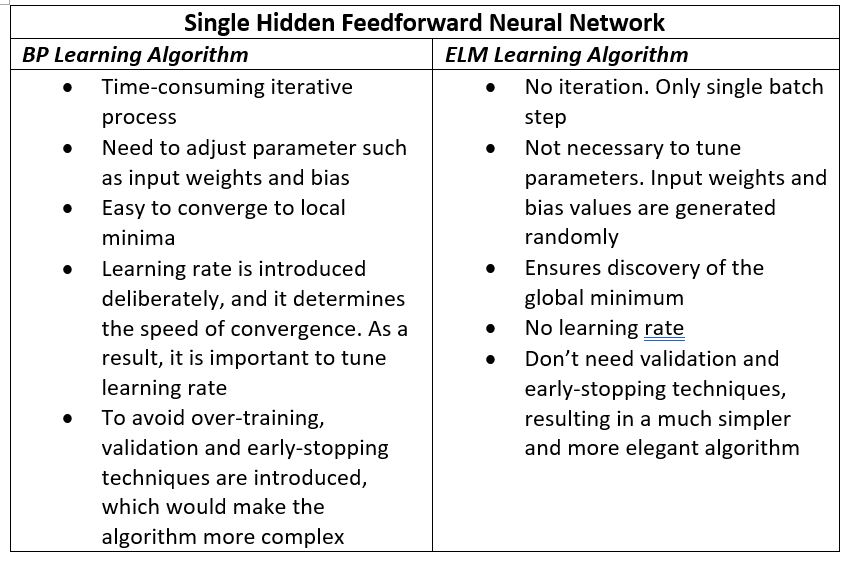
\includegraphics[width=\textwidth]{2.png}
\caption{\label{fig:BP vs ELM}BP algorithm vs. ELM algorithm}
\end{figure}
\subsection{Online Sequential ELM}
\par The basic ELM algorithm processes all training data in batch mode. It works in a static data setting scenario. But in the streaming data setting scenario, the training data comes one by one or chunk by chunk like a time series. This kind of data streaming is also referred to as online sequential data. G.B. Huang et al. in 2005 and N.Y. Liang et al. in 2006 proposed an extended ELM algorithm for online sequential data, which is called Online Sequential ELM(OSELM)
\cite{huang2005line}\cite{liang2006fast}. The OSELM can learn the data one by one or chunk by chunk with fixed or varying sizes\cite{huang2015trends}. The following is the OSELM algorithm:\cite{huang2015trends}\cite{liang2006fast}
\newline \par
\begin{algorithm}[H]
\SetAlgoLined
\SetKwInOut{Input}{input}
\SetKwInOut{Output}{output}
\BlankLine
\KwData{Given an $\textsl{\textbf{initial}}$ training set $\aleph$ = \{\((\mathbf{x}_i,\mathbf{t}_i) \vert \mathbf{x}_i \in \mathbf{R}^n, \mathbf{t}_i \in \mathbf{R}^m, i=1,...,N\)\}}  N denotes number of instances in the training set. For each instance in \( \mathbf{x}\), there are \(n\) attributes(features). For each class in \( \mathbf{t}\), there are \(m\) labels.
\BlankLine
$\textbf{1. Basic ELM training stage}$
\BlankLine
$\textbf{Initialization:}$ Let \(k = 0\). \newline Use the basic ELM in Algorithm 1 and the initial training set to train an initial ELM model. The initial hidden layer output matrix \(\mathbf{H}_0\) and the estimated initial output weights \(\mathbf{\beta}^{(0)}\) are calculated. Set the initial class vector \(\mathbf{T}\) as \(\mathbf{T}_0\). Let \(\mathbf{P}_0 = (\mathbf{H}^T_0\mathbf{H}_0)^{-1}\)
\BlankLine  
\BlankLine
$\textbf{2. Recursive least-squares updating stage}$
\BlankLine
$\textbf{Recursive Updating:}$ When the \((k+1)\)th chunk of new data \(\{\mathbf{x}_{k+1}, \mathbf{t}_{t+1}\}\) arrives:
\newline
$\textbf{Definition 1:}$ Set the class matrix of the new data chunk as \(\Delta\mathbf{T}_{k+1}\) 
\newline
$\textbf{Definition 2:}$ The partial hidden layer output matrix \(\Delta\mathbf{H}_{k+1}\) for the \((k+1)\)th chunk of data 
\newline
$\textbf{Recursive Calculation:}$ Calculate the output weights \(\mathbf{\beta}^{(k+1)}\)
\newline
\While{Data arriving is true}{
read the data chunk\;
\eIf{(it is the first data chunk)}{
\(\mathbf{P}_1 = \mathbf{P}_0-\mathbf{P}_0{\Delta\mathbf{H}_1}^T(\mathbf{I}+\Delta\mathbf{H}_1\mathbf{P}_0{\Delta\mathbf{H}_1}^T)^{-1}\Delta\mathbf{H}_1\mathbf{P}_0\)\;
\(\mathbf{\beta}^{(1)} = \mathbf{\beta}^{(0)}+\mathbf{P}_1{\Delta\mathbf{H}_1}^T(\Delta\mathbf{T}_{1}-\Delta\mathbf{H}_1\mathbf{\beta}^{(0)})\)\;
set \(k=k+1\)\;
}
{
\(\mathbf{P}_{k+1} = \mathbf{P}_k-\mathbf{P}_k{\Delta\mathbf{H}_{k+1}}^T(\mathbf{I}+\Delta\mathbf{H}_{k+1}\mathbf{P}_k{\Delta\mathbf{H}_{k+1}}^T)^{-1}\Delta\mathbf{H}_{k+1}\mathbf{P}_k\)\;
\(\mathbf{\beta}^{(k+1)} = \mathbf{\beta}^{(k)}+\mathbf{P}_{k+1}{\Delta\mathbf{H}_{k+1}}^T(\Delta\mathbf{T}_{k+1}-\Delta\mathbf{H}_{k+1}\mathbf{\beta}^{(k)})\)\;
set \(k=k+1\)\;
}
\
}
\BlankLine
 \caption{OSELM Algorithm}
\end{algorithm}
The size of data chunk can be fixed to any appropriate integer number or can vary when the training data arrives. It is a special case if the training data arrives one by one. The OSELM algorithm can be proved as follows\cite{liang2006fast}.\newline\newline
$\textbf{The basic ELM training stage}$\newline
\par The basic ELM training process is in batch mode. An initial training data set needs to be available for training. After training, \(\mathbf{H}_0\) and the estimated output weights \(\mathbf{\beta}^{(0)}\) are available. The class matrix \(\mathbf{T}_0\) is already known. According to the Basic ELM algorithm in Algorithm 1, the output weights: \(\mathbf{\beta}^{(0)} = {\mathbf{H}_0}^\dagger\mathbf{T}_0\).
\par \(\mathbf{H}^\dagger\) is the Moore-Penrose generalized inverse of the hidden layer output matrix \(\mathbf{H}\) as discussed in the previous sections. The orthogonal projection method, orthogonalization method, iterative method and singular value decomposition(SVD) method are usually used to calculate the Moore-Penrose generalized inverse. Especially, if \(\mathbf{H}^T\mathbf{H}\) is nonsingular, there is \(\mathbf{H}^\dagger={(\mathbf{H}^T\mathbf{H})}^{-1}\mathbf{H}^T\). As a result, \({\mathbf{H}_0}^\dagger={{(\mathbf{H}_0}^T\mathbf{H}_0)}^{-1}{\mathbf{H}_0}^T\). Let \(\mathbf{K}_0={\mathbf{H}_0}^T\mathbf{H}_0\): 
\begin{equation}
\begin{split}
    \mathbf{\beta}^{(0)} &= {\mathbf{H}_0}^\dagger\mathbf{T}_0 
    \\&= {(\mathbf{H}_0}^T\mathbf{H}_0)^{-1}{\mathbf{H}_0}^T\mathbf{T}_0\\&= (\mathbf{K}_0)^{-1}{\mathbf{H}_0}^T\mathbf{T}_0
\end{split}
\end{equation}
\newline
$\textbf{Recursive updating stage}$\newline
\par It is supposed that there is a new chunk of data arriving. \(\Delta\mathbf{H}_1\) denotes the hidden layer output matrix of the chunk of the data. \(\Delta\mathbf{T}_1\) denotes the class matrix of the chunk of the data. The initial training data set together with the new chunk of data can be regarded as a new whole data set. As a result, for the new whole data set, the hidden layer output matrix can be denoted as \(\mathbf{H}_1\). The class matrix of the new whole data set is \(\mathbf{T}_1\). The new output weights matrix is \(\mathbf{\beta}^{(1)}={\mathbf{H}_1}^\dagger\mathbf{T}_1\) which can be written as follows. 
\begin{equation}
\begin{split}
    \mathbf{\beta}^{(1)}&={\mathbf{H}_1}^\dagger\mathbf{T}_1
    \\&=    
    {(\mathbf{H}_1}^T\mathbf{H}_1)^{-1}{\mathbf{H}_1}^T\mathbf{T}_1
    \\&={\mathbf{K}_1}^{-1}
    \begin{bmatrix}
    &\mathbf{H}_0&\\
    &\Delta\mathbf{H}_1&
    \end{bmatrix}^T
    \begin{bmatrix}
    &\mathbf{T}_0&\\
    &\Delta\mathbf{T}_1&
    \end{bmatrix}
\end{split}
\end{equation}
where
\begin{equation}
    \mathbf{K}_1=
    {\mathbf{H}_1}^T\mathbf{H}_1=
    \begin{bmatrix}
    &\mathbf{H}_0&\\
    &\Delta\mathbf{H}_1&
    \end{bmatrix}^T
    \begin{bmatrix}
    &\mathbf{H}_0&\\
    &\Delta\mathbf{H}_1&
    \end{bmatrix}
\end{equation}
\(\mathbf{K}_1\) can be re-written as follows:
\begin{equation}
\begin{split}
    \mathbf{K}_1 &= \begin{bmatrix}
    &\mathbf{H}_0&\\
    &\Delta\mathbf{H}_1&
    \end{bmatrix}^T
    \begin{bmatrix}
    &\mathbf{H}_0&\\
    &\Delta\mathbf{H}_1&
    \end{bmatrix}
    \\&=
    \begin{bmatrix}
    &{\mathbf{H}_0}^T& {\Delta\mathbf{H}_1}^T&\\
    \end{bmatrix}
    \begin{bmatrix}
    &\mathbf{H}_0&\\
    &\Delta\mathbf{H}_1&
    \end{bmatrix}
    \\&=\mathbf{K}_0+{\Delta\mathbf{H}_1}^{T}\Delta\mathbf{H}_1
\end{split}
\end{equation}
\newline
and
\newline
\begin{equation}
    \begin{split}
      \begin{bmatrix}
    &\mathbf{H}_0&\\
    &\Delta\mathbf{H}_1&
    \end{bmatrix}^T
    \begin{bmatrix}
    &\mathbf{T}_0&\\
    &\Delta\mathbf{T}_1&
    \end{bmatrix}
    &={\mathbf{H}_0}^T\mathbf{T}_0+{\Delta\mathbf{H}_1}^T\Delta\mathbf{T}_1 
    \\&=\mathbf{K}_0{\mathbf{K}_0}^{-1}{\mathbf{H}_0}^T\mathbf{T}_0+{\Delta\mathbf{H}_1}^T\Delta\mathbf{T}_1
    \\&=\mathbf{K}_0\mathbf{\beta}^{(0)}+{
    \Delta\mathbf{H}_1}^T\Delta\mathbf{T}_1
    \\&=(\mathbf{K}_1-{\Delta\mathbf{H}_1}^T\Delta\mathbf{H}_1){\mathbf{\beta}}^{(0)}+{\Delta\mathbf{H}_1}^T\Delta\mathbf{T}_1
    \\&=\mathbf{K}_1\mathbf{\beta}^{(0)}-{\Delta\mathbf{H}_1}^T\Delta\mathbf{H}_1{\mathbf{\beta}}^{(0)}+{\Delta\mathbf{H}_1}^T\Delta\mathbf{T}_1
    \end{split}
\end{equation}
\newline
Referring to Equation (15) and Equation (18), \(\mathbf{\beta}^{(1)}\) is solved as follows:
\begin{equation}
    \begin{split}
       \mathbf{\beta}^{(1)}
    &={\mathbf{K}_1}^{-1}
    \begin{bmatrix}
    &\mathbf{H}_0&\\
    &\Delta\mathbf{H}_1&
    \end{bmatrix}^T
    \begin{bmatrix}
    &\mathbf{T}_0&\\
    &\Delta\mathbf{T}_1&
    \end{bmatrix}  
    \\&={\mathbf{K}_1}^{-1}(\mathbf{K}_1\mathbf{\beta}^{(0)}-{\Delta\mathbf{H}_1}^T\Delta\mathbf{H}_1{\mathbf{\beta}}^{(0)}+{\Delta\mathbf{H}_1}^T\Delta\mathbf{T}_1)
    \\&=\mathbf{\beta}^{(0)}+{\mathbf{K}_1}^{-1}{\Delta\mathbf{H}_1}^T(\Delta\mathbf{T}_1-\Delta\mathbf{H}_1{\mathbf{\beta}}^{(0)})
    \end{split}
\end{equation}
\newline
where \(\mathbf{K}_1\) is given in Equation (17).
\newline
\par With reference to Equation (17) and Equation (19), when the \((k+1)\)th chunk of data set is arriving, the following recursive equations can be used for updating the output weights.
\begin{equation}
\begin{split}
    \mathbf{K}_{k+1}&=\mathbf{K}_{k}+{\Delta\mathbf{H}_{k+1}}^T\Delta\mathbf{H}_{k+1}\\
    \mathbf{\beta}^{(k+1)}&=\mathbf{\beta}^{(k)}+{\mathbf{K}_{k+1}}^{-1}{\Delta\mathbf{H}_{k+1}}^T(\Delta\mathbf{T}_{k+1}-\Delta\mathbf{H}_{k+1}{\mathbf{\beta}}^{(k)})
\end{split}
\end{equation}
\newline
Let \(\mathbf{P}_{k+1} = {\mathbf{K}_{k+1}}^{-1}\), and according to the Woodbury formula\cite{GoluVanl96}:
\newline
\begin{equation}
    \begin{split}
        {\mathbf{K}_{k+1}}^{-1} &= (\mathbf{K}_{k}+{\Delta\mathbf{H}_{k+1}}^T\Delta\mathbf{H}_{k+1})^{-1}
        \\&={\mathbf{K}_{k}}^{-1}-{\mathbf{K}_{k}}^{-1}{\Delta\mathbf{H}_{k+1}}^T(\mathbf{I}+\Delta\mathbf{H}_{k+1}{\mathbf{K}_{k}}^{-1}{\Delta\mathbf{H}_{k+1}}^T)^{-1}\\& \quad \times\Delta\mathbf{H}_{k+1}{\mathbf{K}_{k}}^{-1}
    \end{split}
\end{equation}
\newline
Equation (20) can be re-written as:
\newline
\begin{equation}
\begin{split}
  \mathbf{P}_{k+1} &= \mathbf{P}_k-\mathbf{P}_k{\Delta\mathbf{H}_{k+1}}^T(\mathbf{I}+\Delta\mathbf{H}_{k+1}\mathbf{P}_k{\Delta\mathbf{H}_{k+1}}^T)^{-1}\Delta\mathbf{H}_{k+1}\mathbf{P}_k \\
\mathbf{\beta}^{(k+1)} &= \mathbf{\beta}^{(k)}+\mathbf{P}_{k+1}{\Delta\mathbf{H}_{k+1}}^T(\Delta\mathbf{T}_{k+1}-\Delta\mathbf{H}_{k+1}\mathbf{\beta}^{(k)})  
\end{split}
\end{equation}
\newline
Equation (22)\cite{liang2006fast} are the recursive equations in Algorithm 2. 
\newline
\par The OSELM algorithm only needs an initial training data set, as long as the size of the initial data set is larger than the number of the hidden layer neural units. When a new chunk of data arrives, the newest output weights can be updated by the new chunk of the data set based on the previous output weights. This mechanism keeps the output weights updated to the newest incoming data set. 
\subsection{Other Types of ELM and applications}
\par Many ELM variants have been developed, which are extensions of the basic ELM or the OSELM. These ELM variants are applied in different situations. This section briefly introduces some important ELM variants. 
\subsubsection{Incremental ELM}
\par It is acknowledged that the number of hidden layer neural units plays a crucial role in ELM training. It determines the accuracy and the speed of the ELM training and testing. The only parameter needed to be adjusted is the number of the hidden layer neural units for conventional ELMs. Some researchers proposed Incremental ELM that can automatically determine the number of the hidden neuron (architecture) of the SLFN\cite{huang2006universal}\cite{huang2007convex}\cite{zhang2011extreme}. The basic idea is to add hidden neurons one by one to the existing SLFN to test the training error criteria. Only the one that passes the criteria can be kept in the SLFN. By this mechanism, an optimized number of hidden neurons is expected. The Incremental ELM algorithm is a way to construct SLFN, thus saving time to tune the number of hidden neurons manually. 
\subsubsection{OSELM with forgetting mechanism}
\par In some practical applications such as financial market forecasting or weather forecasting,  the data set is a timeline and has a valid period. The older the data is, the more useless it is. It implies that a forgetting mechanism is necessary for such applications to discard older data. OSELM with forgetting mechanism is expected to have higher accuracy and shorter training time. J. Zhao etc. proposed an algorithm based on this idea called FOS-ELM in 2012\cite{zhao2012online}. 
\subsubsection{Other ELM variants}
There are also other ELM variants covering different applications, such as ELM for imbalanced data\cite{HORATA201331}\cite{Zhou2012SurfaceRB}, ELM for noisy/missing data\cite{HORATA201331}\cite{MAN20112491}, ELM ensembles, ELM for semi-supervised learning and ELM for unsupervised learning. These are reviewed in the paper\cite{huang2015trends}.
\subsection{Criticism of ELM}
There are some severe criticisms of the ELM algorithm. Yann LeCun posted a comment in his Facebook account\cite{YannLecun}. He commented: "an ELM is exactly what Minsky \& Papert calls a Gamba Perceptron (a Perceptron whose first layer is a bunch of linear threshold units). The original 1958 Rosenblatt perceptron was an ELM in that the first layer was randomly connected". He also thought it is not appropriate to connect the first layer randomly. He pointed out that it might be effective because there is only one hidden layer, but its applications would be limited and could only be applied in a very narrow area, for example, simple classification problems with small data sets. Dave Chen Pao even wrote a letter to IEEE SMC Exco members to declare that the ELM was a scandal\cite{DaveChenPao}. G.B. Huang wrote a letter to defend himself\cite{Huang2015}. Most of the criticism is mainly concerned about re-inventing the wheel, which means using a new name for an already existing algorithm. 
\newpage
\section{Implementation}
\par As mentioned in the Introduction section, ELMs have been applied in two major data set scenarios: static data setting and streaming data setting. To verify ELMs, we developed two implementations: the basic ELM and the online sequential ELM. The basic ELM is implemented within the WEKA framework and is verified in the static data setting. The online sequential ELM is implemented within the MOA framework and is verified in streaming data setting. The programming language used in the implementation is JAVA. 
\subsection{The basic ELM} 
\par The Waikato Environment for Knowledge Analysis (WEKA) was developed by the Machine Learning group of the University of Waikato. It is a toolbox containing a collection of machine learning algorithms. WEKA can fulfil the tasks of data preparation, classification, regression, clustering, rule mining, as well as visualization \cite{hall2009weka}. Researchers can also extend WEKA by developing a plugin. For example, the deep learning plugin allows WEKA to be extended to support deep learning algorithms. Furthermore, researchers can implement a new algorithm inside the WEKA framework to investigate and evaluate the new algorithm. 
\par The basic ELM is implemented inside the WEKA framework by using Algorithm 1 in section 2.3.2. The basic ELM WEKA implementation is a classifier, which extends AbstractClassifier in WEKA. There are several adjustable parameters. 
\begin{itemize}

\item m\_numHiddenNeurons - The number of neuron units in the hidden layer is critical so that the implementation makes the number of the hidden neutron as an adjustable parameter. 
\item m\_seed - A seed for randomly generating input weights and the values of bias is also adjustable. 
\item m\_typeOfActivation - Because the basic ELM can use many different activation functions, which was indicated in section 2.3.1, the implementation also can change the activation function. By default, the activation function is the Sigmoid function. 
    
\end{itemize}
Please refer to \url{https://github.com/WanliHuang/ELM-WEKA} for the source code. 

\par The basic ELM WEKA version commandline parameters are:
\begin{itemize}
    \item -node  to define the number of the hidden neuron
    \item -activation to define the activation function
    \item -seed  an integer number for generating random numbers
    \item -type to define the type of ELM
    \item -debug the switch of debug mode 
\end{itemize}
A typical WEKA commandline example for the basic ELM WEKA version is:\newline\newline
-t covtype\_train.arff -T covtype\_test.arff -type 1 -seed 1  -node 200 -debug 0 -activate 1
\subsection{Online Sequential ELM}
\par Massive Online Analysis(MOA) is similar to WEKA, whereas it is applied in a streaming data setting. It has a collection of machine learning algorithms, while it is also a framework for data stream mining\cite{MOA}. The online sequential ELM (OSELM) MOA version is implemented within the MOA framework according to Algorithm 2, shown in section 2.4. 
\par As per the basic ELM WEKA implementation, the OSELM MOA version has some adjustable parameters. 
\begin{itemize}
    \item HiddenNeuronNuber - the number of neuron units of the hidden layer
    \item DatasetInitialSize - the number of instances of the initial dataset
    \item isDataChunkFixed - the coming data chunk size is fixed or variable. If the size is fixed, then the size of the chunk data can be set as well
    \item RandomSeed - to randomly generate input weights or bias values
    \item ActivationFunction - can set the type of activation function. The default activation function is Sigmoid Function
\end{itemize}
Please refer to \url{https://github.com/WanliHuang/OS-ELM-MOA} for the source code.

\par The OSELM MOA version commandline parameters are:
\begin{itemize}
    \item n   to determine the number of hidden neurons
    \item s   to determine the size of the initial dataset
    \item c   to determine the size of the chunk of data
    \item s   to determine of seed for generating random numbers
    \item a   to determine the type of ELM
\end{itemize}
A typical MOA commandline for the OSELM MOA version is: \newline\newline
EvaluatePrequential -l functions.OSELM -s (ArffFileStream -f (covtype\_full.arff))
\subsection{Difference between the OSELM implementation and the OSELM Algorithm}
\par There is some difference between the actual implementation of OSELM and the OSELM algorithm, which was shown in Algorithm 2 in section 2.4. 
\par In Algorithm 2, only after all the new data coming to the OSELM has been trained to update the output weights will new data be used for testing. As a result, each new incoming data is tested using the most up to date output weights. 
\par In the OSELM implementation, all new data is used for training to update the output weights. Meanwhile, the new data is also used for testing. It means the most updated output weights are always for the next incoming data. 
\newpage
\section{Experiments}
In this section, the performance of the basic ELM and the Online Sequence ELM(OSELM) are evaluated by reproducing results from the literature as well as being compared with popular machine learning algorithms on some benchmark 
classification datasets. The basic ELM is evaluated in a static data setting, while the OSELM is tested in a streaming data setting.
\subsection{Experiment Settings}
\par 
The computer configuration used for all experiments is as follows:
\begin{itemize}

    \item CPU: Intel Core i7-7700HQ 2.80GHz
    \item RAM: 8G
    \item Operation System: Windows10 Laptop

\end{itemize}
\par To test the basic ELM, for a specific benchmark problem, we use two datasets in arff format. The first one is the training dataset; the second one is the testing dataset. To test OSELM, we use prequential evaluation as the evaluation method. We also use the arff format dataset. All input attributes and output classes are normalized in the experiments. 
\subsection{Performance Evaluation}
\subsubsection{Basic ELM performance}
\par \textbf{(1). Small size classification problem} \newline\newline
     The experiment was conducted for a real classification problem: Pima Indians Diabetes Database, which was produced in the Applied Physics Laboratory, Johns Hopkins University, 1988. The dataset can be downloaded from Kaggle \url{https://www.kaggle.com}. The dataset contains the medical records for Pima Indian patients, showing whether a patient has signs of diabetes or not. There are eight attributes and 1 class for each sample. The class is binary valued: 1 for positive and 0 for negative. The size of the dataset is 768 instances. 75\% of the samples are chosen for the training dataset, and the remainder is used for testing. \newline\newline
     The performance of the Basic ELM on the Diabetes dataset is summarized as follows.
     \begin{figure}[H]
\centering
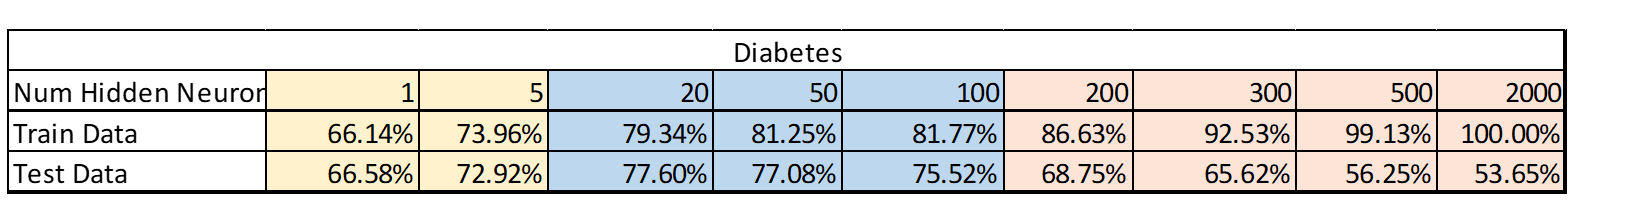
\includegraphics[width=1.1\textwidth]{3_1.png}
\caption{\label{fig:Diabetes}Pima Indians Diabetes Database}
\end{figure}

When the number of hidden neurons is 20, the result is similar to what G.B Huang et al. claim. In the paper\cite{G.B.Huang-ICNN}, the accuracy rate for the training set is 78.71\%, and the accuracy rate for the testing dataset is 76.54\%. 
     \begin{figure}[H]
\centering
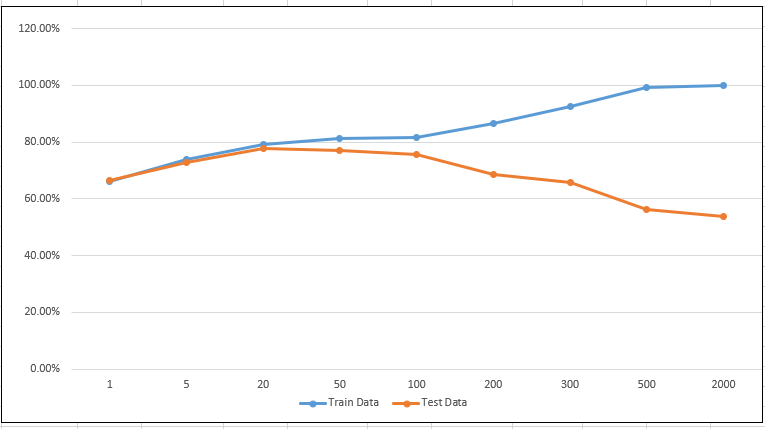
\includegraphics[width=\textwidth]{4.png}
\caption{\label{fig:trainingvstesting}Diabetes training dataset vs. testing dataset}
\end{figure}
 From Figure 5,  when the number of hidden neurons is below 20, it is underfitting, whereas, when the number is greater than 100, it is overfitting.\newline 
\par\textbf{(2). Large size classification problem}\newline\newline
This experiment was carried out on a much larger dataset: Forest Cover Type Prediction, which was provided by the US Forest Service Region 2 Resource Information System. The dataset can be downloaded from Kaggle as well. The cover type dataset size is extremely large. There are 581012 samples(instances). Each sample has 54 attributes and 1 class. The class has 7 labels, representing 7 types of forest cover designation. 10000 instances are chosen randomly as the training dataset, the remaining 481012 instances are used for testing. The performance of the basic ELM on Forest Cover Type dataset is summarized as below:
\begin{figure}[H]
\centering
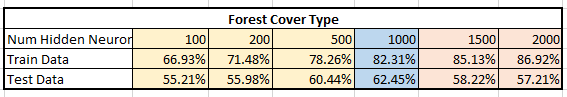
\includegraphics[width=\textwidth]{5.png}
\caption{\label{fig:trainingvstesting}Forest Cover Type dataset}
\end{figure}
The performance is worse than reported in the literature. In the paper\cite{G.B.Huang-ICNN}, the accuracy rate for the training set is 92.35\% and the accuracy rate for the testing dataset is 90.21\% when the number of hidden neurons is 200.  The basic ELM WEKA version performance could not therefore be substantiated. In the paper \cite{G.B.Huang-ICNN}, the Forest Cover Type dataset was revised into a binary classification problem. The performance results in the paper \cite{G.B.Huang-ICNN} are for the binary classification problem. To evaluate using the same assumptions, a revised Forest Cover Type dataset, which has a binary class value, is introduced into the experiment. Meanwhile, the ELM Matlab version is also obtained from the ELM office website \url{https://www.ntu.edu.sg/home/egbhuang/elm_codes.html}. The ELM Matlab version is also used for comparison. The performances of the basic ELM WEKA version and the basic ELM Matlab version on the revised Forest Cover Type dataset are summarized in the tables below.
\begin{figure}[H]
\centering
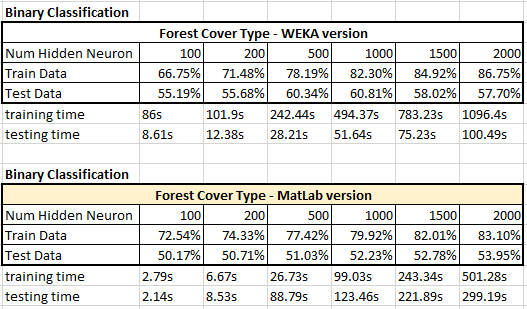
\includegraphics[width=\textwidth]{6.png}
\caption{\label{fig:trainingvstesting}Forest Cover Type dataset with binary class values}
\end{figure}
From Figure 7, the WEKA and the MatLab versions both
produce results that are worse than those claimed in the paper\cite{G.B.Huang-ICNN}.\newline 
%\par\textbf{(3). Benchmark Experiments}\newline\newline%
\subsubsection{Basic ELM Benchmark Experiments}
Additional datasets were selected for benchmark experiments. There are six binary and six multi-class classification problems in the benchmarks. The specifications of each dataset are described in Table 1 and Table 2. \newline\newline
\begin{table}[H]
\caption{Specifications of Benchmark datasets - Binary Classification Problem}
\label{tab:binarydatasets}
\centering
\begin{tabular}{ |p{3cm}||p{2.5cm}|p{2.5cm}|p{2.5cm}|p{2.5cm}|  }
 \hline
 \multicolumn{5}{|c|}{Binary Class Data sets} \\
 \hline
 Dataset Name& Attributes & Instances &  Training Data & Testing Data\\
 \hline
  Adult income& 14  & 48842 &30000&   18842\\
 \hline
 Airlines   & 7    & 539383 & 234156 &   305227\\
  \hline
 Australian Credit&   14  & 690   & 488 &   202\\
  \hline
 Banana & 2 & 5300 &  3052&  2248\\
   \hline
 Diabetes &   8 & 768 & 500 &   268 \\
  \hline
 Electricity &   8 & 45312 &19989&   25323\\
  \hline
 Liver disorders& 7  & 345 &123&   222\\
  \hline
  Spambase & 57  & 4601 &3600&1001\\ 
 \hline
   Tic-Tac-Toe & 9  & 958 &700&258\\ 
 \hline
\end{tabular}
\end{table}

\begin{table}[H]
\caption{Specifications of Benchmark datasets - Multi-class Classification Problem}
\label{tab:multidatasets}
\centering
\begin{tabular}{ |p{2.8cm}||p{2cm}|p{2cm}|p{2cm}|p{2cm}|p{2cm}|  }
 \hline
 \multicolumn{6}{|c|}{Multi-Classes Data sets} \\
 \hline
 Dataset Name& Attributes & Instances &  Training Data & Testing Data & Number of Class\\
 \hline
 Ecoli   & 7    & 336 & 200  &  136  & 8\\
  \hline
 Glass Identification&   9  &  214  & 150 &  64  & 7\\
  \hline
 Iris & 4 & 150 & 100 &  50  & 3\\
  \hline
 Satellite Image   &36 & 6435 &  4000 &  2435  & 7\\
  \hline
 Vehicle silhouettes & 18  & 946   & 600 &  346 & 4\\
  \hline 
 Vowel & 14  & 990 &  600 &  390  &11\\
  \hline
\end{tabular}
\end{table}
\par For the binary classification problems in Table~\ref{tab:binarydatasets}, ten machine learning algorithms are chosen to compare with the basic ELM. They are MultilayerPerceptron, NaiveBayes, AdaBoostM1, MultiClassClassifier, ZeroR, HoeffdingTree, J48, RandomForest, RandomTree and SGD. These were chosen as a broad but representative set of methods. Each method uses WEKA default parameters. Evaluation is by 10 by 10-fold cross-validation.
Table \ref{tab:binaryRank} below shows the ranking of these eleven algorithms.
\newline\newline
Experiment Type: 10 times 10 fold cross-validation \newline
Tester:     weka.experiment.PairedCorrectedTTester \newline
Analysing:  Percent\_correct \newline
Datasets:   6 \newline
Resultsets: 11 \newline
Confidence: 0.05 (two tailed) \newline
Sorted by:  Percent\_correct

\begin{table}[thb]
\caption{\label{tab:binaryRank}Machine Learning Algorithm Resultsets Ranking  - Binary Classification}
\footnotesize
{\centering \begin{tabular}{rllll}\\
\hline
Resultset (ML algorithm) & Wins$-$ & Wins & Losses& Rank  \\
& Losses & & & \\
\hline
trees.RandomForest &  37 &  39 &   2 &1\\
trees.J48 &  24 &  30 &   6 &2\\
 functions.MultilayerPerceptron&  17 &  25 &   8  &3\\
meta.MultiClassClassifier &  16 &  25 &   9 &4\\
 functions.SGD&  15 &  24 &   9 &5\\
meta.AdaboostM1 &   4 &  21 &  17 &6\\
trees.RandomTree &  -7 &  22 &  29 &7\\
function.ExtremeLearningMachine & -11 &  16 &  27 &8\\
trees.HoeffdingTree & -13 &  13 &  26 &9\\
 bayes.NaiveBayes& -26 &  10 &  36 &10\\
rules.ZeroR & -56 &   0 &  56  &11\\
\hline
\end{tabular} \footnotesize \par}
\end{table}
Table \ref{tab:EML-base} shows the ELM-based cross validation experiments' details. The figures in Table \ref{tab:EML-base} are percent of correct classification with standard deviations for each machine learning algorithm on each data set. The symbol $\circ$ attached to a figure presents the fact that a machine learning algorithm shows a statistically significant improvement compared to the basic ELM. The symbol $\bullet$ attached to a figure means a statistically significant degradation compared to basic ELM. If a figure is without a symbol it means there is no statistically significant difference. Table \ref{tab:emlbaseKeys} shows keys for Table \ref{tab:EML-base} and the configurations for each machine learning algorithm. 
\par It is concluded that the basic ELM's performance is relatively poor, obtaining an overall rank of 8, and located in the lower range in Table \ref{tab:binaryRank}. The basic ELM wins 16 trials and loses 27 trials. The net loss is 11 trials, compared to other machine learning algorithms.  
\par Unfortunately, due to out of memory error, the basic ELM was not able to conduct experiments on three datasets: Adult income, Airlines and Electricity. Essentially, the sizes of these three datasets are too large for the basic ELM to handle. 
\begin{landscape}
\begin{table}[thb]
\caption{\label{tab:EML-base}Machine Learning Algorithms Comparison Details - ELM base - Binary Classification}
\scriptsize
{\centering \begin{tabular}{lr@{\hspace{0cm}}c@{\hspace{0cm}}rr@{\hspace{0cm}}c@{\hspace{0cm}}r@{\hspace{0.1cm}}cr@{\hspace{0cm}}c@{\hspace{0cm}}r@{\hspace{0.1cm}}cr@{\hspace{0cm}}c@{\hspace{0cm}}r@{\hspace{0.1cm}}cr@{\hspace{0cm}}c@{\hspace{0cm}}r@{\hspace{0.1cm}}cr@{\hspace{0cm}}c@{\hspace{0cm}}r@{\hspace{0.1cm}}cr@{\hspace{0cm}}c@{\hspace{0cm}}r@{\hspace{0.1cm}}cr@{\hspace{0cm}}c@{\hspace{0cm}}r@{\hspace{0.1cm}}cr@{\hspace{0cm}}c@{\hspace{0cm}}r@{\hspace{0.1cm}}cr@{\hspace{0cm}}c@{\hspace{0cm}}r@{\hspace{0.1cm}}cr@{\hspace{0cm}}c@{\hspace{0cm}}r@{\hspace{0.1cm}}c}
\\
\hline
Dataset & \multicolumn{3}{c}{(1)}& \multicolumn{4}{c}{(2)} & \multicolumn{4}{c}{(3)} & \multicolumn{4}{c}{(4)} & \multicolumn{4}{c}{(5)} & \multicolumn{4}{c}{(6)} & \multicolumn{4}{c}{(7)} & \multicolumn{4}{c}{(8)} & \multicolumn{4}{c}{(9)} & \multicolumn{4}{c}{(10)} & \multicolumn{4}{c}{(11)} \\
\hline
australian & 67.19 & $\pm$ & 5.78 & 83.07 & $\pm$ & 4.07 &   $\circ$ & 77.33 & $\pm$ & 4.03 &   $\circ$ & 84.80 & $\pm$ & 3.79 &   $\circ$ & 84.64 & $\pm$ & 3.97 &   $\circ$ & 85.30 & $\pm$ & 3.73 &   $\circ$ & 55.51 & $\pm$ & 0.67 & $\bullet$ & 85.23 & $\pm$ & 3.77 &   $\circ$ & 85.61 & $\pm$ & 3.65 & $\circ$ & 86.68 & $\pm$ & 3.71 & $\circ$ & 78.81 & $\pm$ & 5.40 &   $\circ$\\
tic-tac-toe & 68.17 & $\pm$ & 2.54 & 97.39 & $\pm$ & 1.45 &   $\circ$ & 69.64 & $\pm$ & 4.40 &           & 98.33 & $\pm$ & 1.28 &   $\circ$ & 72.72 & $\pm$ & 4.12 &   $\circ$ & 98.28 & $\pm$ & 1.36 &   $\circ$ & 65.34 & $\pm$ & 0.41 & $\bullet$ & 69.64 & $\pm$ & 4.40 &           & 85.28 & $\pm$ & 3.18 & $\circ$ & 96.78 & $\pm$ & 1.94 & $\circ$ & 79.83 & $\pm$ & 4.94 &   $\circ$\\
liver-disorders & 71.80 & $\pm$ & 7.67 & 68.73 & $\pm$ & 7.38 &           & 54.89 & $\pm$ & 8.83 & $\bullet$ & 67.57 & $\pm$ & 7.32 &           & 65.96 & $\pm$ & 7.11 &           & 68.72 & $\pm$ & 7.98 &           & 57.98 & $\pm$ & 0.84 & $\bullet$ & 55.98 & $\pm$ & 6.44 & $\bullet$ & 65.84 & $\pm$ & 7.40 &         & 73.23 & $\pm$ & 7.97 &         & 64.10 & $\pm$ & 7.71 & $\bullet$\\
spambase & 76.14 & $\pm$ & 2.11 & 90.99 & $\pm$ & 3.04 &   $\circ$ & 79.56 & $\pm$ & 1.56 &   $\circ$ & 92.40 & $\pm$ & 1.03 &   $\circ$ & 90.03 & $\pm$ & 1.62 &   $\circ$ & 92.57 & $\pm$ & 1.17 &   $\circ$ & 60.60 & $\pm$ & 0.09 & $\bullet$ & 79.23 & $\pm$ & 2.52 &   $\circ$ & 92.68 & $\pm$ & 1.08 & $\circ$ & 95.54 & $\pm$ & 0.92 & $\circ$ & 91.13 & $\pm$ & 1.49 &   $\circ$\\
pima-diabetes & 76.76 & $\pm$ & 4.55 & 74.75 & $\pm$ & 4.90 &           & 75.75 & $\pm$ & 5.32 &           & 77.31 & $\pm$ & 4.69 &           & 74.92 & $\pm$ & 4.80 &           & 77.47 & $\pm$ & 4.39 &           & 65.11 & $\pm$ & 0.34 & $\bullet$ & 75.72 & $\pm$ & 5.35 &           & 74.49 & $\pm$ & 5.27 &         & 76.10 & $\pm$ & 4.49 &         & 70.25 & $\pm$ & 4.55 & $\bullet$\\
banana & 86.44 & $\pm$ & 2.12 & 72.36 & $\pm$ & 2.38 & $\bullet$ & 61.32 & $\pm$ & 1.70 & $\bullet$ & 55.17 & $\pm$ & 0.09 & $\bullet$ & 69.14 & $\pm$ & 3.06 & $\bullet$ & 55.84 & $\pm$ & 1.97 & $\bullet$ & 55.17 & $\pm$ & 0.09 & $\bullet$ & 68.74 & $\pm$ & 5.42 & $\bullet$ & 89.07 & $\pm$ & 1.22 & $\circ$ & 89.09 & $\pm$ & 1.32 & $\circ$ & 87.22 & $\pm$ & 1.34 &          \\
\hline
\multicolumn{33}{c}{$\circ$, $\bullet$ statistically significant improvement or degradation}\\
\end{tabular} \scriptsize \par}
\end{table}


\begin{table}[thb]
\caption{\label{tab:emlbaseKeys}Key, configurations of each machine learning algorithm}
\scriptsize
{\centering
\begin{tabular}{cl}\\
(1) & functions.ExtremeLearningMachine '-debug 0 -node 20 -seed -1 -activate 1 -type 1' -4253773317834344110 \\
(2) & functions.MultilayerPerceptron '-L 0.3 -M 0.2 -N 500 -V 0 -S 0 -E 20 -H a' -5990607817048210779 \\
(3) & bayes.NaiveBayes '' 5995231201785697655 \\
(4) & functions.SGD '-F 0 -L 0.01 -R 1.0E-4 -E 500 -C 0.001 -S 1' -3732968666673530290 \\
(5) & meta.AdaBoostM1 '-P 100 -S 1 -I 10 -W trees.DecisionStump' -1178107808933117974 \\
(6) & meta.MultiClassClassifier '-M 0 -R 2.0 -S 1 -W functions.Logistic -- -R 1.0E-8 -M -1 -num-decimal-places 4' -3879602011542849141 \\
(7) & rules.ZeroR '' 48055541465867954 \\
(8) & trees.HoeffdingTree '-L 2 -S 1 -E 1.0E-7 -H 0.05 -M 0.01 -G 200.0 -N 0.0' 7117521775722396251 \\
(9) & trees.J48 '-C 0.25 -M 2' -217733168393644444 \\
(10) & trees.RandomForest '-P 100 -I 100 -num-slots 1 -K 0 -M 1.0 -V 0.001 -S 1' 1116839470751428698 \\
(11) & trees.RandomTree '-K 0 -M 1.0 -V 0.001 -S 1' -9051119597407396024 \\
\end{tabular}
}
\end{table}
\end{landscape}
\par For the multi-class classification problems in Table \ref{tab:multidatasets}, ten machine learning algorithms are chosen to compare with the basic ELM. They are MultilayerPerceptron, NaiveBayes, AdaBoostM1, MultiClassClassifier, ZeroR, HoeffdingTree, J48, RandomForest, RandomTree and LogitBoost. Chosen as before to represent a broad selection of methods. Table \ref{tab:multiRank} below shows the ranking of these eleven algorithms.
\newline\newline
Experiment Type: 10 times 10 folds Cross-validation \newline
Tester:     weka.experiment.PairedCorrectedTTester \newline
Analysing:  Percent\_correct \newline
Datasets:   6 \newline
Resultsets: 11 \newline
Confidence: 0.05 (two tailed) \newline
Sorted by:  Percent\_correct

\begin{table}[thb]
\caption{\label{tab:multiRank}Machine Learning Algorithm Resultsets Ranking  - Multi-class Classification}
\footnotesize
{\centering \begin{tabular}{rllll}\\
\hline
Resultset(ML algorithm) & Wins$-$ & Wins & Losses & Rank\\
& Losses & & &\\
\hline
trees.RandomForest &  38 &  40 &   2 & 1\\
funtions.MultilayerPerceptron &  33 &  36 &   3 & 2\\
trees.J48 &  18 &  25 &   7 & 3\\
meta.LogitBoost &  15 &  25 &  10 & 4\\
meta.MultiClassClassifier &  14 &  25 &  11 & 5\\
trees.RandomTree&   8 &  24 &  16 & 6\\
functions.ExtremeLearningMachine &  -5 &  15 &  20 & 7\\
trees.HoeffdingTree & -12 &  13 &  25 & 8\\
bayes.NavieBayes & -12 &  13 &  25 & 9\\
meta.AdaboostM1 & -37 &   6 &  43 & 10\\
rules.ZeroR & -60 &   0 &  60 & 11\\
\hline
\end{tabular} \footnotesize \par}
\end{table} 
Table \ref{tab:multi-EML-base} shows the ELM-based cross validation experiments' details. Symbols $\circ$ and $\bullet$ have the same meaning as in Table \ref{tab:EML-base}. In Table \ref{tab:multiRank},  the basic ELM is ranked 7th, winning 15 trials and losing 20 trials (a net loss of 5 trials), compared to other machine learning algorithms. It shows only modest performance. 
\par For both binary class classification and multi-class classification, the basic ELM shows generally poor performance. The best out-of-the-box machine learning algorithm is clearly Random Forest.  
\begin{landscape}
\begin{table}[thb]
\caption{\label{tab:multi-EML-base}Machine Learning Algorithms Comparison Details- ELM base - Multi-class Classification}
\scriptsize
{\centering \begin{tabular}{lr@{\hspace{0cm}}c@{\hspace{0cm}}rr@{\hspace{0cm}}c@{\hspace{0cm}}r@{\hspace{0.1cm}}cr@{\hspace{0cm}}c@{\hspace{0cm}}r@{\hspace{0.1cm}}cr@{\hspace{0cm}}c@{\hspace{0cm}}r@{\hspace{0.1cm}}cr@{\hspace{0cm}}c@{\hspace{0cm}}r@{\hspace{0.1cm}}cr@{\hspace{0cm}}c@{\hspace{0cm}}r@{\hspace{0.1cm}}cr@{\hspace{0cm}}c@{\hspace{0cm}}r@{\hspace{0.1cm}}cr@{\hspace{0cm}}c@{\hspace{0cm}}r@{\hspace{0.1cm}}cr@{\hspace{0cm}}c@{\hspace{0cm}}r@{\hspace{0.1cm}}cr@{\hspace{0cm}}c@{\hspace{0cm}}r@{\hspace{0.1cm}}cr@{\hspace{0cm}}c@{\hspace{0cm}}r@{\hspace{0.1cm}}c}
\\
\hline
Dataset & \multicolumn{3}{c}{(1)}& \multicolumn{4}{c}{(2)} & \multicolumn{4}{c}{(3)} & \multicolumn{4}{c}{(4)} & \multicolumn{4}{c}{(5)} & \multicolumn{4}{c}{(6)} & \multicolumn{4}{c}{(7)} & \multicolumn{4}{c}{(8)} & \multicolumn{4}{c}{(9)} & \multicolumn{4}{c}{(10)} & \multicolumn{4}{c}{(11)} \\
\hline
ecoli & 82.61 & $\pm$ & 15.58 & 84.86 & $\pm$ & 5.55 &         & 85.50 & $\pm$ & 5.46 &           & 64.62 & $\pm$ & 1.94 & $\bullet$ & 86.50 & $\pm$ & 5.49 &         & 42.56 & $\pm$ & 1.18 & $\bullet$ & 83.81 & $\pm$ &  5.94 &           & 82.86 & $\pm$ & 5.70 &         & 85.69 & $\pm$ & 5.15 &         & 78.94 & $\pm$ & 6.60 &         & 83.78 & $\pm$ & 4.95 &        \\
Glass & 61.74 & $\pm$ & 10.66 & 67.32 & $\pm$ & 8.64 &         & 49.45 & $\pm$ & 9.50 & $\bullet$ & 44.89 & $\pm$ & 3.05 & $\bullet$ & 64.26 & $\pm$ & 8.25 &         & 35.51 & $\pm$ & 2.15 & $\bullet$ & 47.80 & $\pm$ & 10.29 & $\bullet$ & 67.58 & $\pm$ & 9.30 &         & 79.72 & $\pm$ & 8.72 & $\circ$ & 68.97 & $\pm$ & 9.84 &         & 70.99 & $\pm$ & 8.64 & $\circ$\\
iris & 95.80 & $\pm$ &  4.51 & 96.93 & $\pm$ & 4.07 &         & 95.53 & $\pm$ & 5.02 &           & 95.40 & $\pm$ & 5.74 &           & 96.07 & $\pm$ & 4.55 &         & 33.33 & $\pm$ & 0.00 & $\bullet$ & 95.27 & $\pm$ &  5.47 &           & 94.73 & $\pm$ & 5.30 &         & 94.67 & $\pm$ & 5.01 &         & 93.27 & $\pm$ & 4.97 &         & 94.93 & $\pm$ & 4.75 &        \\
satellite-image & 63.63 & $\pm$ &  1.50 & 89.43 & $\pm$ & 1.10 & $\circ$ & 79.59 & $\pm$ & 1.60 &   $\circ$ & 43.80 & $\pm$ & 0.37 & $\bullet$ & 83.59 & $\pm$ & 0.89 & $\circ$ & 23.82 & $\pm$ & 0.08 & $\bullet$ & 79.61 & $\pm$ &  1.60 &   $\circ$ & 86.41 & $\pm$ & 1.18 & $\circ$ & 91.77 & $\pm$ & 0.87 & $\circ$ & 85.26 & $\pm$ & 1.26 & $\circ$ & 85.67 & $\pm$ & 1.24 & $\circ$\\
vehicle & 70.91 & $\pm$ &  4.59 & 81.14 & $\pm$ & 3.86 & $\circ$ & 44.68 & $\pm$ & 4.59 & $\bullet$ & 39.81 & $\pm$ & 1.80 & $\bullet$ & 79.04 & $\pm$ & 4.00 & $\circ$ & 25.51 & $\pm$ & 0.51 & $\bullet$ & 45.45 & $\pm$ &  4.44 & $\bullet$ & 72.28 & $\pm$ & 4.32 &         & 74.87 & $\pm$ & 3.87 &         & 70.05 & $\pm$ & 4.48 &         & 70.73 & $\pm$ & 4.05 &        \\
vowel & 32.69 & $\pm$ &  4.19 & 92.72 & $\pm$ & 3.08 & $\circ$ & 62.90 & $\pm$ & 4.38 &   $\circ$ & 17.47 & $\pm$ & 0.82 & $\bullet$ & 65.19 & $\pm$ & 4.19 & $\circ$ &  9.09 & $\pm$ & 0.00 & $\bullet$ & 62.87 & $\pm$ &  4.39 &   $\circ$ & 80.20 & $\pm$ & 4.36 & $\circ$ & 98.10 & $\pm$ & 1.54 & $\circ$ & 82.99 & $\pm$ & 3.98 & $\circ$ & 70.96 & $\pm$ & 4.75 & $\circ$\\
\hline
\multicolumn{33}{c}{$\circ$, $\bullet$ statistically significant improvement or degradation}\\
\end{tabular} \scriptsize \par}
\end{table}


\begin{table}[thb]
\caption{\label{tab:m-emlbaseKeys}Key for configurations of each machine learning algorithm}
\scriptsize
{\centering
\begin{tabular}{cl}\\
(1) & functions.ExtremeLearningMachine '-debug 0 -node 20 -seed -1 -activate 1 -type 1' -4253773317834344110 \\
(2) & functions.MultilayerPerceptron '-L 0.3 -M 0.2 -N 500 -V 0 -S 0 -E 20 -H a' -5990607817048210779 \\
(3) & bayes.NaiveBayes '' 5995231201785697655 \\
(4) & meta.AdaBoostM1 '-P 100 -S 1 -I 10 -W trees.DecisionStump' -1178107808933117974 \\
(5) & meta.MultiClassClassifier '-M 0 -R 2.0 -S 1 -W functions.Logistic -- -R 1.0E-8 -M -1 -num-decimal-places 4' -3879602011542849141 \\
(6) & rules.ZeroR '' 48055541465867954 \\
(7) & trees.HoeffdingTree '-L 2 -S 1 -E 1.0E-7 -H 0.05 -M 0.01 -G 200.0 -N 0.0' 7117521775722396251 \\
(8) & trees.J48 '-C 0.25 -M 2' -217733168393644444 \\
(9) & trees.RandomForest '-P 100 -I 100 -num-slots 1 -K 0 -M 1.0 -V 0.001 -S 1' 1116839470751428698 \\
(10) & trees.RandomTree '-K 0 -M 1.0 -V 0.001 -S 1' -9051119597407396024 \\
(11) & meta.LogitBoost '-P 100 -L -1.7976931348623157E308 -H 1.0 -Z 3.0 -O 1 -E 1 -S 1 -I 10 -W trees.DecisionStump' -1105660358715833753 \\
\end{tabular}
}
\end{table}

\end{landscape}



\subsubsection{OSELM performance}
\par MOA can use the arff dataset format to simulate a data stream to evaluate a machine learning algorithm. It just requires the dataset size to be large enough. In this experiment, the Forest Cover Type dataset is chosen as its size is considerable. There are 581012 instances, 53 features, and seven types of class. To stimulate the real data stream setting, we adopt the prequential evaluation method. The experiment is to verify the performance claim in the paper\cite{liang2006fast}. 

\par The experiment results are shown in Figure \ref{fig:OSELMCOVTYPE}. It is a two-dimension table. The row values are the number of hidden neurons. The column values are the size of the initial dataset. The chunk data size is fixed to 1, which means the training and testing are done instance by instance. The accuracy is increased when the number of hidden neurons increases. After the number of hidden neurons reaches 300, the accuracy increases slow. Furthermore, they start to drop when the number of hidden neurons reaches 450. The processing time increases together with increasing the number of hidden neurons. When the number of hidden neurons is 400, and the size of the initial dataset is 1000, the accuracy is the highest, at 74.56\%. The processing time of the whole arff file data stream is 3 hours, 12 minutes and 35 seconds.
 \par If the initial size is fixed to 1000 and the hidden neuron number is fixed to 20, only the data chunk size is variable. The experiment's results are summarized in Figure \ref{fig:OSELMCHUNKSIZE}. The chunk size doesn't impact the result, but it increases the experiment processing time.
\par Figure \ref{fig:HeoTree-HoeAdaptive} shows the results of the experiments that use HoeffdingTree and HoeffingAdaptiveTree.
\par HeoffdingTree and HoeffingAdaptiveTree are built-in MOA machine learning algorithms. In these experiments, HoeffdingTree and HoeffingAdaptiveTree both adopt default settings. It is obvious that both HoeffdingTree and HoeffingAdaptiveTree have much higher accuracy and are much faster. Figure \ref{fig:OSELM}, Figure \ref{fig:HeoffdingTree}, Figure \ref{fig:HeoffdingTreeAdaptive} and Figure \ref{fig:OSELMvsHOEFFDINGTREE} give more details of the experiments. 
\begin{landscape}
\begin{figure}[H]
\centering
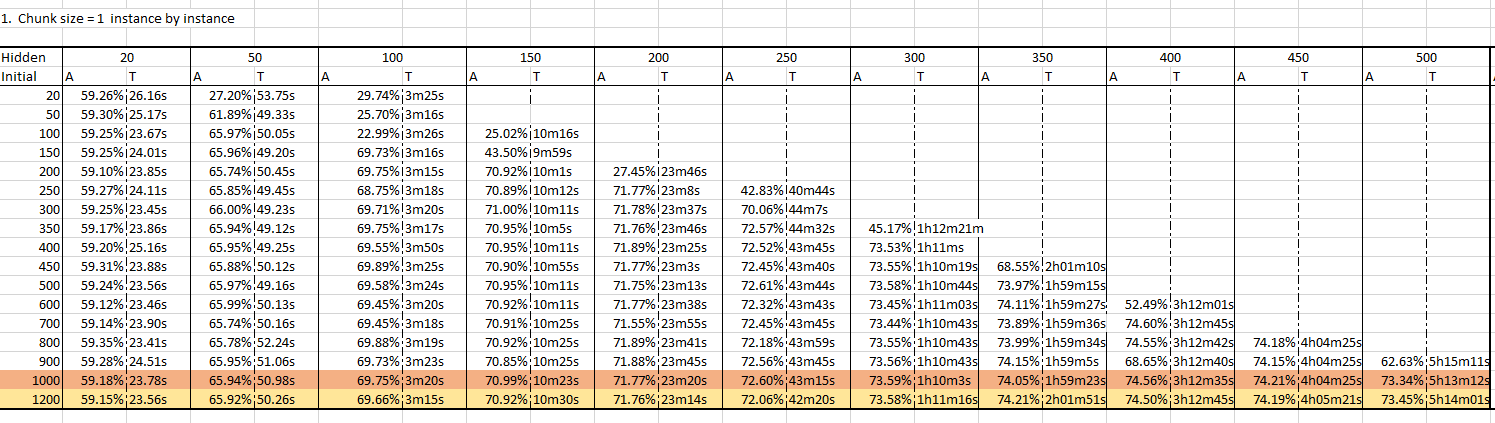
\includegraphics[width=1.4\textwidth]{7.png}
\caption{\label{fig:OSELMCOVTYPE}Forest Cover Type dataset, prequential valuation, OSELM. In the table, A stands for accuracy, T for experiment time}
\end{figure}
\end{landscape}

 \begin{figure}[H]
\centering
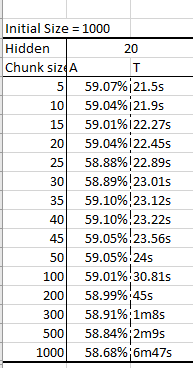
\includegraphics[width=0.4\textwidth]{8.png}
\caption{\label{fig:OSELMCHUNKSIZE}OSELM, Forest Cover Type, variable chunk size. In the table, A stands for accuracy, T for experiment time }
\end{figure}
  
 \begin{figure}[H]
\centering
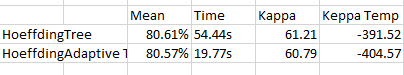
\includegraphics[width=\textwidth]{9.png}
\caption{\label{fig:HeoTree-HoeAdaptive}HoeffdingTree and HoeffingAdaptiveTree, Forest Cover Type}
\end{figure}

\begin{landscape}
 \begin{figure}[H]
\centering

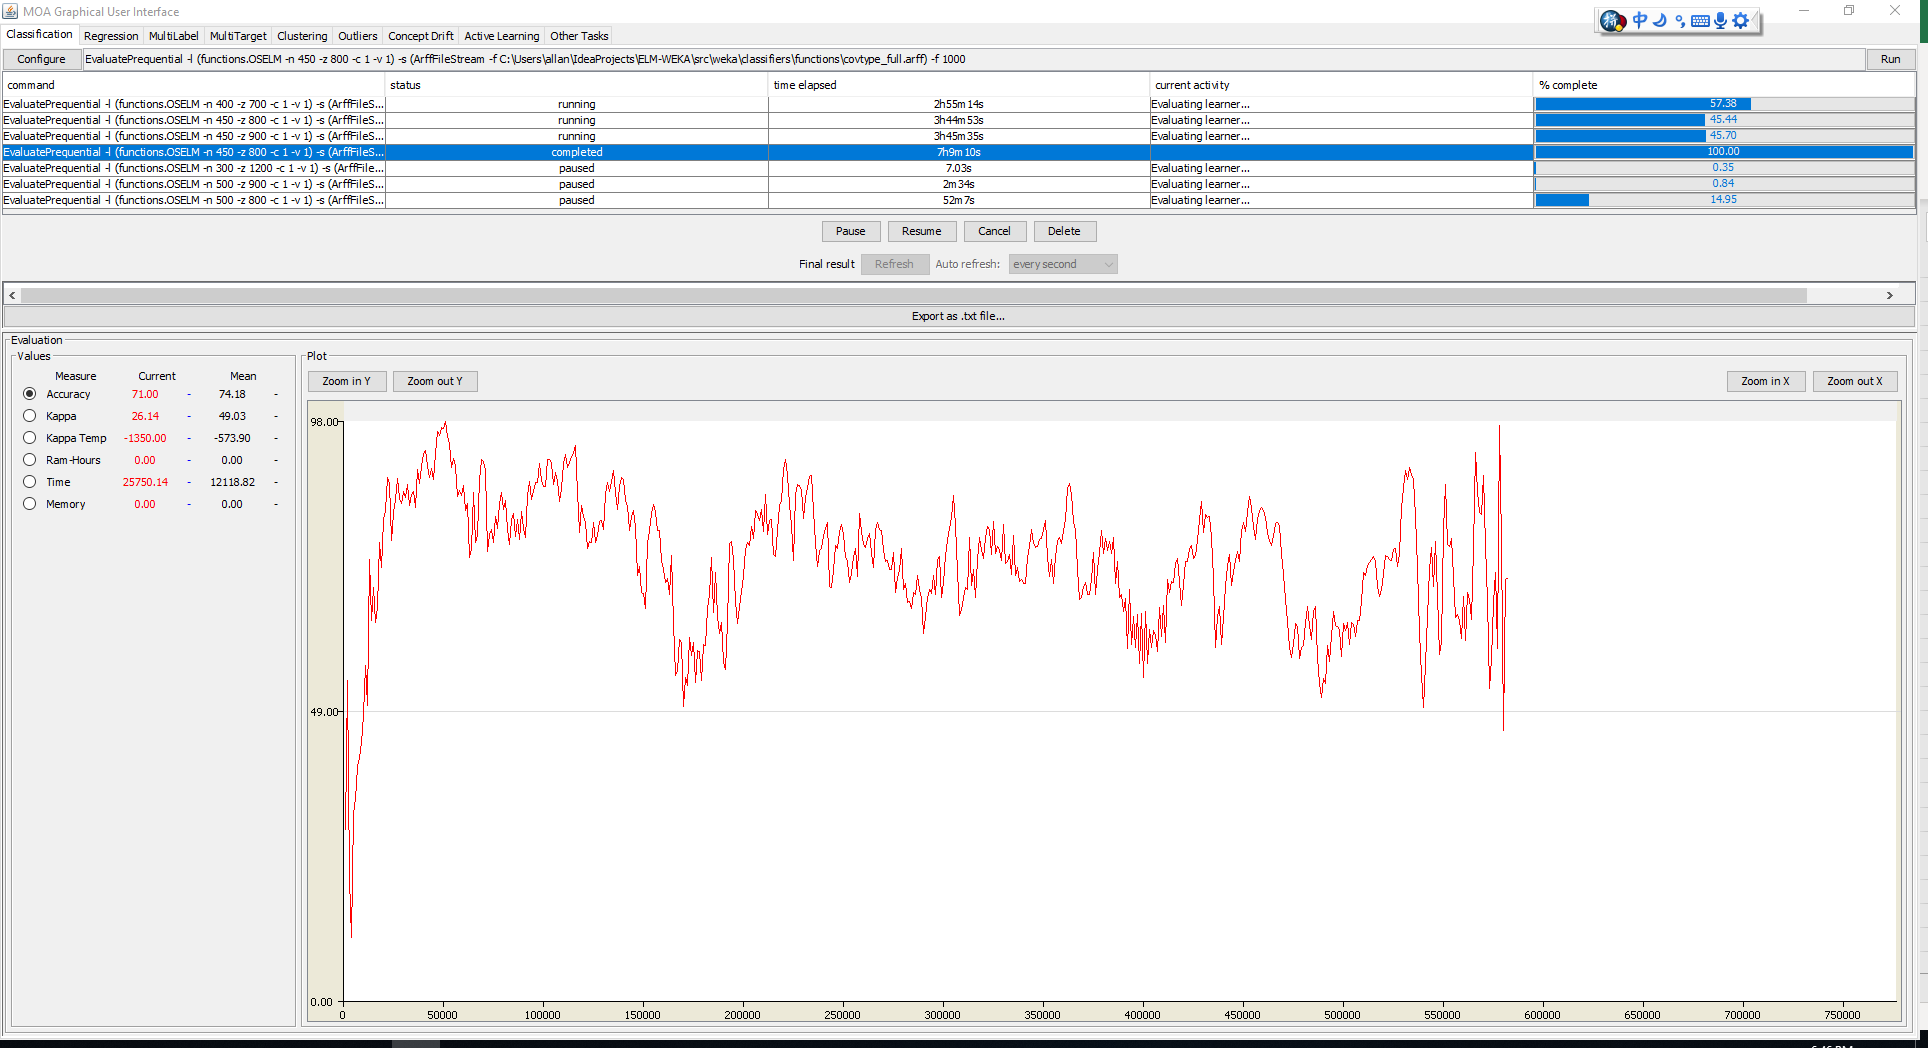
\includegraphics[width=1.35\textwidth]{11.png}
\caption{\label{fig:OSELM}OSELM: Initial size 800, Chunk size 1, hidden neuron number 450, sample frequency 1000. Arff file data stream: Forest Cover Type}
\end{figure}
 \begin{figure}[H]
\centering
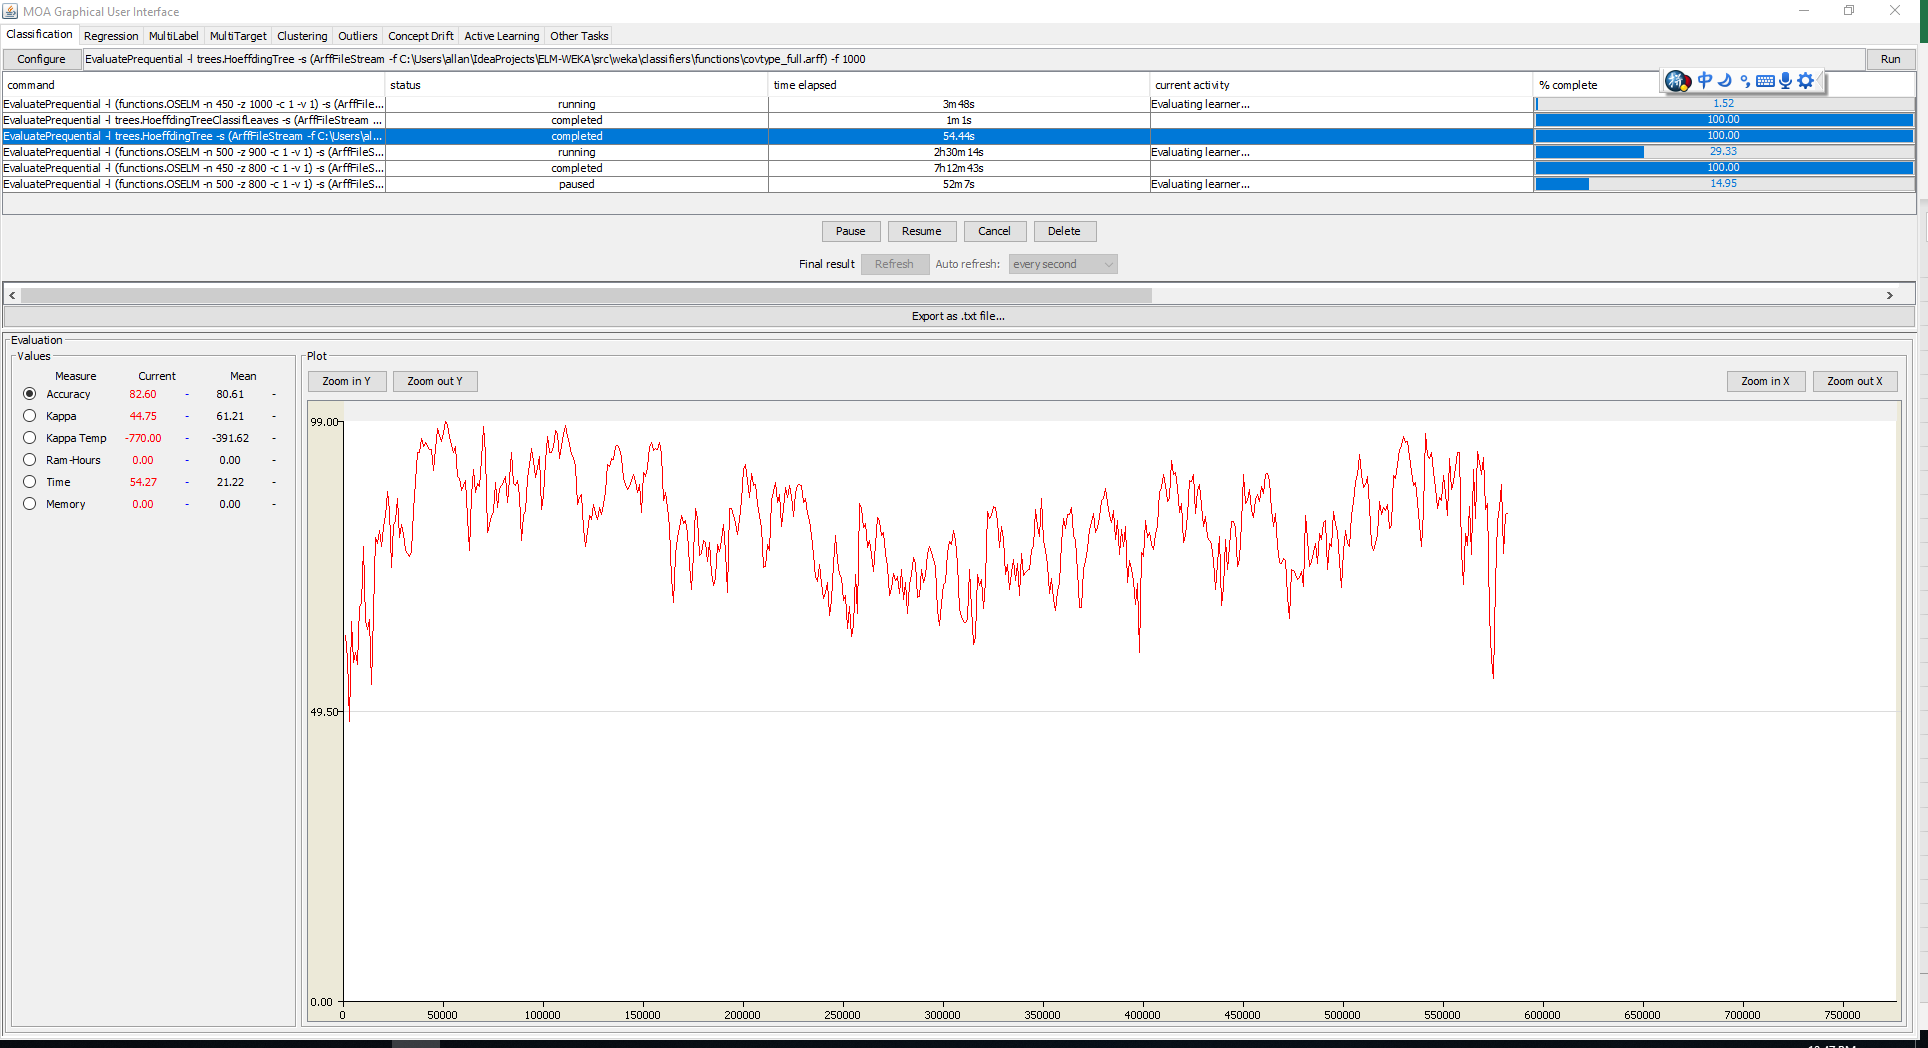
\includegraphics[width=1.35\textwidth]{13.png}
\caption{\label{fig:HeoffdingTree} HoeffdingTree,  MOA default parameters, Arff file data stream: Forest Cover Type}
\end{figure}
 \begin{figure}[H]
\centering
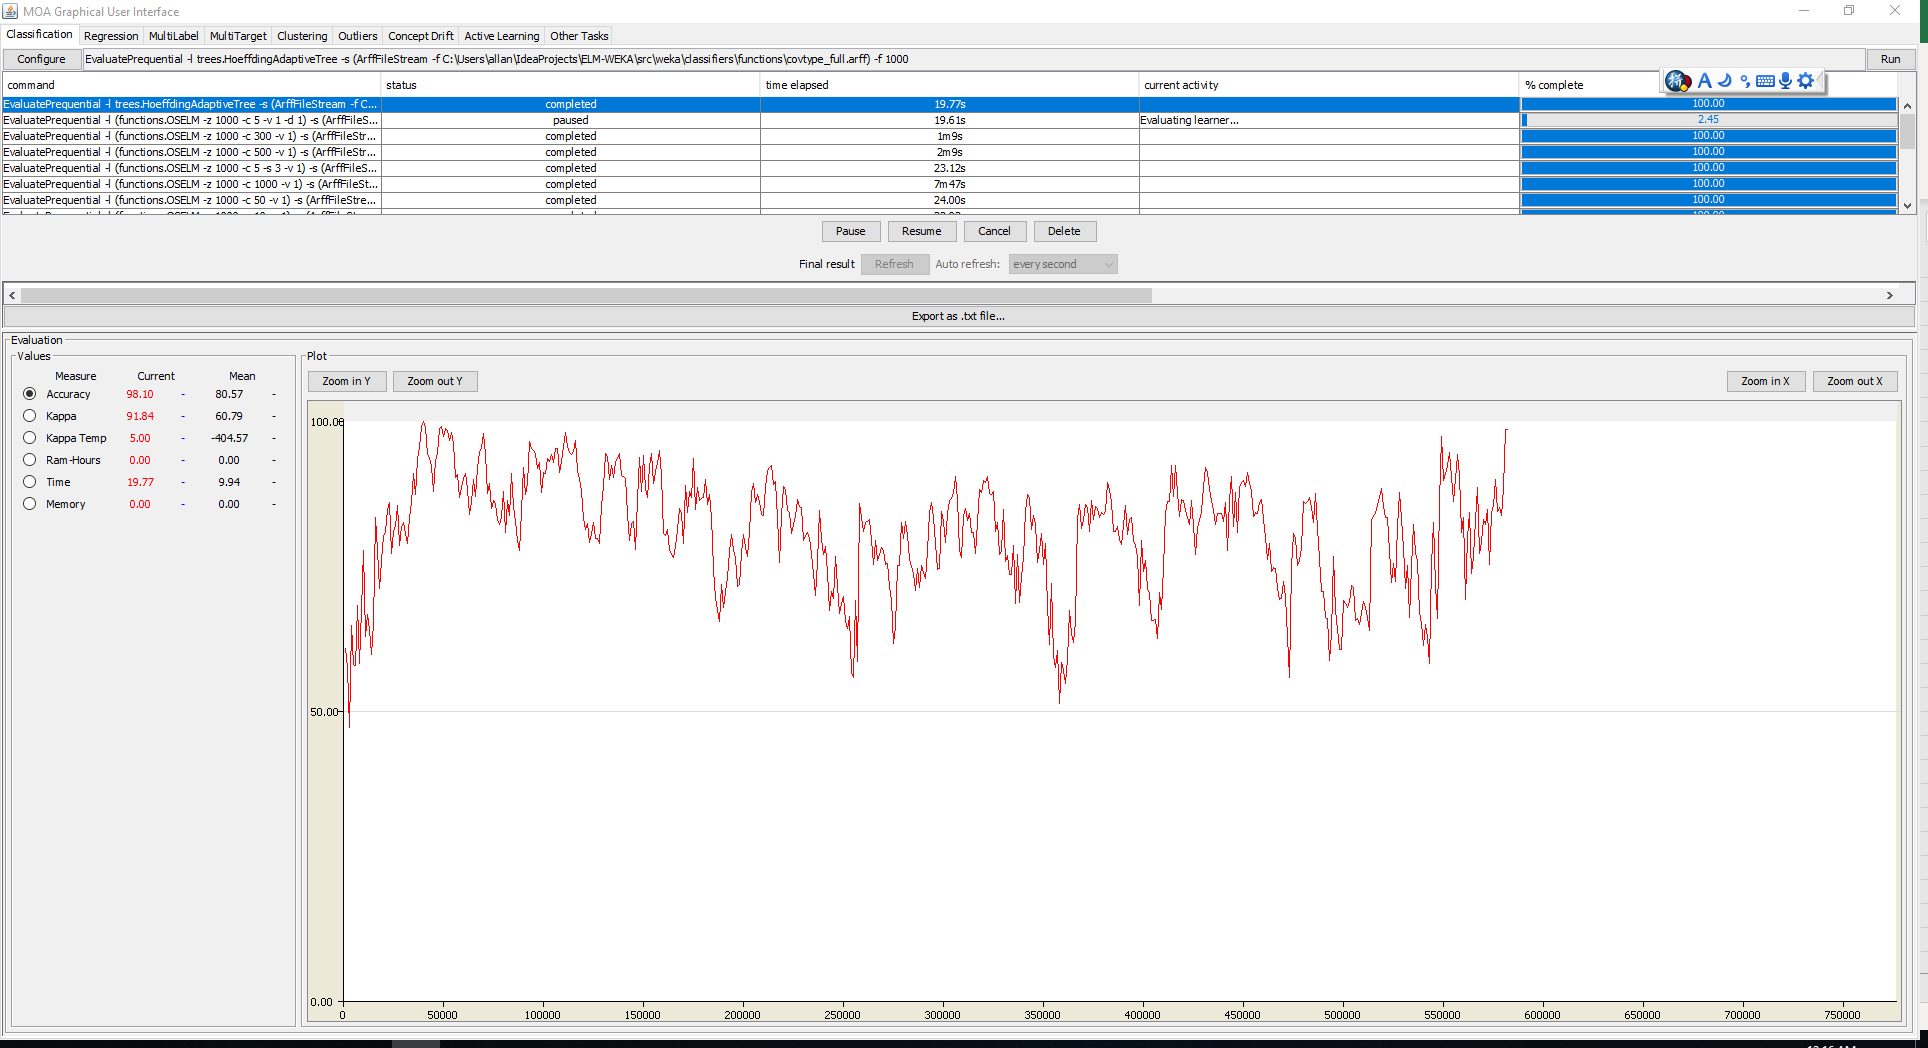
\includegraphics[width=1.35\textwidth]{12.png}
\caption{\label{fig:HeoffdingTreeAdaptive}HoeffdingTreeAdaptive, MOA default parameters, Arff file data stream: Forest Cover Type}
\end{figure}
 \begin{figure}[H]
\centering
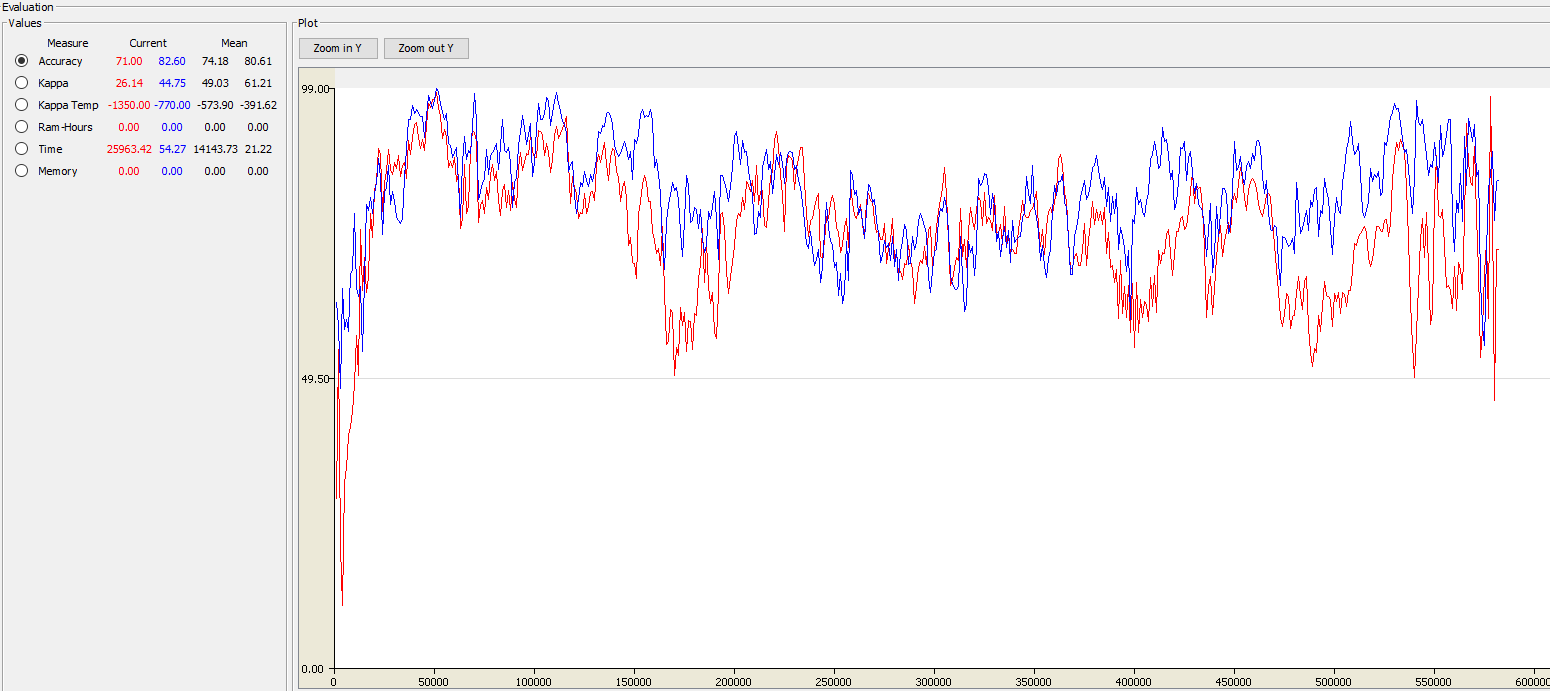
\includegraphics[width=1.35\textwidth]{10.png}
\caption{\label{fig:OSELMvsHOEFFDINGTREE}OSELM vs. HoeffdingTree, Forest Cover Type}
\end{figure}
\textbf{Red line:} OSELM MOA version  \textbf{Blue line:}HoeffdingTree
\end{landscape}
\par Figure \ref{fig:OSELM} shows that the average accuracy of the OSELM MOA version is 74.18\%. The whole processing time of the arff file data stream is 4 hours 4 minutes and 24 seconds (refer to Figure \ref{fig:OSELMCOVTYPE}). The maximum accuracy it can reach is 98\%, and the minimum accuracy is 15\%. Figure 12 shows that the HoeffdingTree average accuracy is 80.61\%. The maximum accuracy is 99\%, and the minimum accuracy is 49\%. The HoeffdingTree has better performance than the OSELM MOA version. Regarding training and testing speed, HoeffdingTree is much faster than the OSELM MOA version. The processing time of the arff file data stream is 54.44 seconds. Figure 13 shows that the HeoffdingAdaptiveTree average accuracy is 80.57\%. The maximum accuracy is 99\%, and the minimum accuracy is 49\%. The speed is even faster. The processing time of the arff file data stream is 19.77 seconds. Figure 14 shows the comparison of OSELM to the HoeffdingTree. The OSELM MOA version does not show any adavantages, compared to either the HoeffdingTree or the HoeffdingAdaptiveTree.   
\subsubsection{OSELM Benchmark Experiments}

\par\textbf{1. Multiple Machine Learning Algorithms on a Single Dataset}
\newline
\par We chose ten machine learning algorithms together with OSELM to do experiments on the same data stream. They are Oza Bag, ruleClassifier, Naive Bayes, Hoeffding Adaptive Tree, Hoeffding Tree, Oza Boost, KNN, SGD MultiClass, Perceptron, and Random Forest. The Random Forest Covtype dataset is used in MOA to generate the data stream. OSELM's configuration uses 200 hidden neurons, an initial dataset size of 1000, and data chunk size of 1. The ranks of percent of correct are shown in Table \ref{tab:OSELMCovtRank}. OSELM's rank is 7, showing relatively poor performance, but the processing time is the longest one. Figure \ref{fig:benchmark screenshots} is the MOA screenshots of the ten algorithms' experiments.  It also shows OSELM is not as stable as SGDMultiClass, KNN and OzaBoost.
\newline
\newline
\textbf{2. Cross Validation and Significance test on Multi-datasets}
\newline

\par In order to obtain a more precise evaluation, we also chose 9 machine learning algorithms to compare with OSELM. They are AdaptiveRandomForest, HoeffdingAdaptiveTree, KNN, NaiveBayes, OzaBoost, Perceptron, RuleClassifier, SGDmultiClassifier and WeightedMajority. Meanwhile, we chose two MOA stream generators: ConceptDriftRealStream and PartitioningStream.  We also selected three Arff format datasets to generate data streams. They are summarized in Table \ref{tab:OSELMCV}.
\begin{table}[thb]
\caption{\label{tab:OSELMCovtRank}Machine Learning Algorithm Ranking  - Dataset: Covtype arff }
\footnotesize
{\centering \begin{tabular}{rllll}\\
\hline
ML algorithm & Mean Accuracy (percent) & Mean Kappa & Processing Time & Rank\\

\hline
functions.SGDMultiClass & 93.41 & 87.67  &   6.62s & 1\\
lazy.KNN &  92.23 &  84.72 &   8m33s & 2\\
meta.OzaBoost &  90.86 &  81.15 &   20m40s & 3\\
meta.OzaBag &  84.61 &  68.54 &  10m36s & 4\\
trees.HoeffdingTree &  80.61 &  61.21 &  52.64s & 5\\
trees.HoeffdingTree &   80.57 &  60.79 &  31.86s & 6\\
functions.OSELM &  72.60 &  44.83 &  1h10m49s & 7\\
rules.ruleClassifier & 60.32 &  16.26 &  5m34s & 8\\
bayes.NaiveBayes & 57.66 &  16.89 &  15.20s & 9\\
WEKAClassifier.RandomForrest & 57.64 &   23.46 &  1m9s & 10\\
function.perceptron & 48.68 &   0.00 &  6.16s & 11\\
\hline
\end{tabular} \footnotesize \par}
\end{table}
\begin{figure}
    \centering
    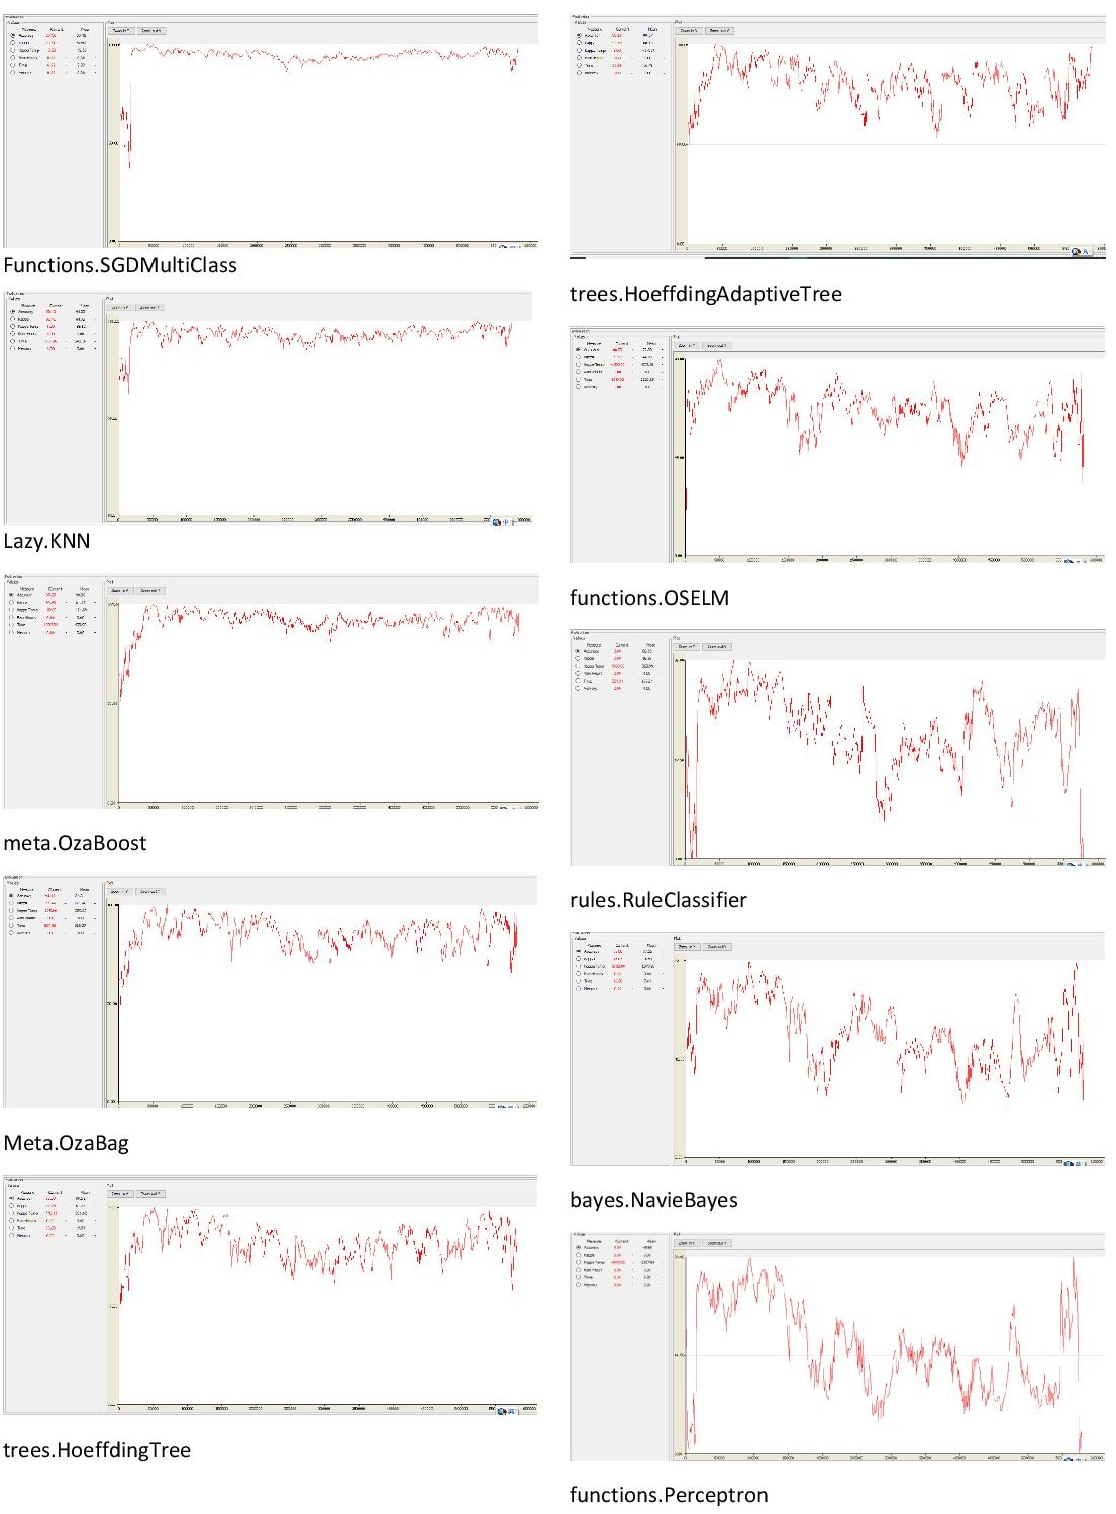
\includegraphics[width=\textwidth]{OSELM-benchmark.jpg}
    \caption{Benchmark Experiments Screenshots}
    \label{fig:benchmark screenshots}
\end{figure}

\begin{table}[H]
\caption{Specifications of Benchmark datasets}
\label{tab:OSELMCV}
\centering
\begin{tabular}{ |p{2.8cm}||p{2.5cm}|p{2.5cm}|p{2.5cm}|  }
 \hline
 Dataset Name& Attributes & Instances &   Number of Class\\
 \hline
 Covertype   &  53   & 581012 &  7\\
  \hline
 Electricity &   9  &  45321  & 2\\
  \hline
 GMSC & 10 & 150000 & 2\\
  \hline
\end{tabular}
\end{table}
\par The following are the setup of the cross validation experiments
\newline
\newline Evaluation Type: class.moa.EvaluatePrequentialCV  \newline
Significance Test: Statistic T-test     \newline
Analysing:  Percent\_correct \newline
Data stream:   5 \newline
Confidence: 0.05 (two tailed) \newline

\begin{landscape}
\begin{table}[thb]
\caption{\label{tab:OSELM-CV-details}Nine Machine Learning Algorithms Compared to OSELM on five data streams}
\scriptsize
{\centering \begin{tabular}{lr@{\hspace{0cm}}c@{\hspace{0cm}}rr@{\hspace{0cm}}c@{\hspace{0cm}}r@{\hspace{0.1cm}}cr@{\hspace{0cm}}c@{\hspace{0cm}}r@{\hspace{0.1cm}}cr@{\hspace{0cm}}c@{\hspace{0cm}}r@{\hspace{0.1cm}}cr@{\hspace{0cm}}c@{\hspace{0cm}}r@{\hspace{0.1cm}}cr@{\hspace{0cm}}c@{\hspace{0cm}}r@{\hspace{0.1cm}}cr@{\hspace{0cm}}c@{\hspace{0cm}}r@{\hspace{0.1cm}}cr@{\hspace{0cm}}c@{\hspace{0cm}}r@{\hspace{0.1cm}}cr@{\hspace{0cm}}c@{\hspace{0cm}}r@{\hspace{0.1cm}}cr@{\hspace{0cm}}c@{\hspace{0cm}}r@{\hspace{0.1cm}}cr@{\hspace{0cm}}c@{\hspace{0cm}}r@{\hspace{0.1cm}}c}
\\
\hline
Dataset & \multicolumn{3}{c}{(1)}& \multicolumn{4}{c}{(2)} & \multicolumn{4}{c}{(3)} & \multicolumn{4}{c}{(4)} & \multicolumn{4}{c}{(5)} & \multicolumn{4}{c}{(6)} & \multicolumn{4}{c}{(7)} & \multicolumn{4}{c}{(8)} & \multicolumn{4}{c}{(9)} & \multicolumn{4}{c}{(10)} \\
\hline
PStream & 69.92 & $\pm$ & 7.14 & 88.16 & $\pm$ & 9.40 & $\circ$        & 94.57 & $\pm$ & 6.03 &  $\circ$    & 76.03 & $\pm$ & 1.61 & $\circ$ & 73.63 & $\pm$ & 1.76 &  $\circ$       & 94.77 & $\pm$ & 10.65 & $\circ$ & 63.03 & $\pm$ &  1.65 & $\bullet$          & 70.29 & $\pm$ & 2.92 &         & 60.29 & $\pm$ & 2.44 &  $\bullet$       & 94.98 & $\pm$ & 5.40 & $\circ$           \\
CStream & 68.86 & $\pm$ & 4.47 & 85.24 & $\pm$ & 12.16 &   $\circ$      & 97.59 & $\pm$ & 3.54 & $\circ$ & 76.02 & $\pm$ & 1.79 & $\circ$ & 69.14 & $\pm$ & 2.10 &   & 92.84 & $\pm$ & 14.83 &$\circ$  & 63.17 & $\pm$ & 2.24 & $\bullet$ & 67.56 & $\pm$ & 2.94 &   & 60.09 & $\pm$ & 2.65 & $\bullet$ & 94.52 & $\pm$ &6.46 &  $\circ$    \\
CType & 72.14 & $\pm$ &  11.95 & 91.95 & $\pm$ & 36.76& $\circ$ & 80.75 & $\pm$ & 72.62 &  $\circ$  & 91.94 & $\pm$ & 21.42 &  $\circ$  & 57.58 & $\pm$ & 238.68 &  $\bullet$       & 90.01 & $\pm$ & 32.89 & $\circ$ & 48.66 & $\pm$ &  445.72 &   $\bullet$        & 93.02 & $\pm$ & 0.61 &  $\circ$       & 92.91 & $\pm$ & 41.17 &  $\circ$       & 79.51 & $\pm$ & 54.42 & $\circ$         \\
GMSC & 66.14 & $\pm$ &  41.14 & 93.25 & $\pm$ & 0.47 & $\circ$ & 92.97 & $\pm$ & 0.57 &   $\circ$ & 93.05 & $\pm$ & 0.62 & $\circ$ & 73.38 & $\pm$ & 71.97 & $\circ$ & 92.13 & $\pm$ & 0.72 & $\circ$ & 78.67 & $\pm$ &  11.59 &   $\circ$ & 93.03 & $\pm$ & 0.62 & $\circ$ & 87.74 & $\pm$ & 2.17 & $\circ$ & 93.02 & $\pm$ & 0.58 & $\circ$ \\
Elec & 71.30 & $\pm$ &  40.15 & 87.81 & $\pm$ & 6.36 & $\circ$ & 82.69 & $\pm$ & 25.36 & $\circ$ & 78.08 & $\pm$ & 13.94 & $\circ$ & 73.18 & $\pm$ & 71.72 &  & 73.38 & $\pm$ & 71.97 &  & 78.67 & $\pm$ &  11.58 & $\circ$ & 73.08 & $\pm$ & 33.82 &  & 57.55 & $\pm$ & 40.91 &  $\bullet$ & 80.65 & $\pm$ & 37.40 &  $\circ$              \\
\hline
\multicolumn{33}{c}{$\circ$, $\bullet$ statistically significant improvement or degradation}\\
\end{tabular} \scriptsize \par}
\end{table}


\begin{table}[thb]
%\caption{\label{tab:OSELMCV}}%
\scriptsize
{\centering
\begin{tabular}{cl}\\
(1) & functions.OSELM \\
(2) & meta.AdaptiveRandomForest  \\
(3) & trees.HoeffdingAdaptiveTree \\
(4) & lazy.KNN \\
(5) & bayes.NativeBayes \\
(6) & meta.OzaBoost \\
(7) & functions.Perceptron \\
(8) & rules.RuleClassifier \\
(9) & functions.SGDMultiClass \\
(10) & meta.WeightedMajorityAlgorithm\\
\\
PStream & PartitioningStream\\
CStream & ConceptDriftRealStream\\
CType & Forest Cover Type dataset arff file stream \\
GMSC & GMSC arff file stream\\
Elec & Electricity arff file stream\\
\end{tabular}
}
\end{table}

\end{landscape}
In this cross validation experiment, OSELM configurations are hidden neurons 200, initial dataset size 1000 and data chunk size 1. The other 9 machine learning algorithms' configurations are set up by default in MOA. After doing pair by pair cross validation experiments and significance t-tests, we have Table \ref{tab:multiRank_datastream} showing the ranking of these 10 machine learning algorithms  as follows:
\newline\newline
Experiment Type: Cross-validation \newline
Evaluation Tester: class.moa.EvaluatePrequentialCV     \newline
Analysing:  Percent\_correct \newline
Datasets:   5 \newline
Resultsets: 10 \newline
Confidence: 0.05 (two tailed) \newline
Sorted by:  Percent\_correct

\begin{table}[thb]
\caption{\label{tab:multiRank_datastream}Machine Learning Algorithm Resultsets Ranking  - Data Stream}
\footnotesize
{\centering \begin{tabular}{rllll}\\
\hline
Resultset(ML algorithm) & Wins$-$ & Wins & Losses & Rank\\
& Losses & & &\\
\hline
meta.WeightedMajorityAlgorithm &  34 & 37  &   3 & 1\\
meta.AdaptiveRandomForest &  29 &  36 &   7 & 2\\
trees.HoefffingAdaptiveTree &  27 &  34 &   7 & 3\\
meta.OzaBoost &  19 &  31 &  12 & 4\\
lazy.KNN &  13 &  27 &  14 & 5\\
rules.RuleClassifier&   -1 &  18 &  19 & 6\\
bayes.NativeBayes &  -19 &  12 &  31 & 7\\
functions.SGDMultiClass & -24 &  9 &  33 & 8\\
functions.OSELM & -25 &  7 &  32 & 9\\
functions.Perceptron & -28 &   8 &  36 & 10\\
\hline
\end{tabular} \footnotesize \par}
\end{table}
\par It is obvious that OSELM isn't competitive among these machine learning algorithms, as it is only ranked at the 9th position. Table \ref{tab:OSELM-CV-details} shows the cross validation results, when OSELM is the test base. 
\newpage
\section{Conclusion}
\par Two major Extreme Learning Machine(ELM) algorithms: the basic ELM and the Online sequential ELM(OSELM) are investigated, implemented and evaluated. The basic ELM WEKA version is implemented within the WEKA framework. The OSELM MOA version is implemented within the MOA framework. Basic ELM is evaluated in the static data setting scenario. OSELM is evaluated in the data stream setting scenario. The performances of the basic ELM WEKA version and the OSELM MOA version are compared to performance levels claimed in the paper\cite{G.B.Huang-ICNN}, as well as with the performance of the Hoeffding Tree and the Hoeffding Adaptive Tree algorithms. 
\par According to the experiments, the basic ELM WEKA version does not show the same (good) result as the one claimed in the paper\cite{G.B.Huang-ICNN}. The performance of the basic ELM WEKA version is moderate at best. The OSELM MOA version does not offer any advantage over either the Hoeffding Tree or the Hoeffding Adaptive Tree. The accuracy is slightly lower than each of them and the speed is significantly slower.
\par Most computer resources, time and computer memory etc, are used for calculating \(\mathbf{H}\) and \(\mathbf{H}^\dagger\). \(\mathbf{H}\) which is a linear function of the number of hidden neurons. It is observed that the time cost increases significantly with the increment of the number of hidden neurons. The number of hidden neurons also determines performance. The performance is worse if the number of hidden neurons is not chosen correctly. On a positive note, ELM does have very few parameters to tune. Because the basic ELM needs to consume a large enough dataset in a batch to learn the model, basic ELM is more suitable for medium to small dataset sizes. 
\par ELM is a learning algorithm. Although G.B. Huang et al. give the learning algorithm a new name, its structure is a single hidden layer feedforward network (SLFN). The renaming is also the main point of the controversial criticism of the method. Replication of results, however, might be another criticism of papers using this or adaptations of this method. 
\par The number of hidden neurons plays a critical role in the ELM algorithm. Research in the future could focus on how to determine this number to obtain an optimized SLFN structure, perhaps using regularization. 
\newpage

\bibliographystyle{plain}
\bibliography{bib.bib}

\end{document}
